O trabalho foi dividido nos quatro passos propostos por S
Du~\cite{s2013automatic}: aquisição da imagem, extração da placa, segmentação dos caracteres e reconhecimento dos caracteres. Na figura \ref{fig:processo} está disposto um exemplo do fluxo a ser seguido

\begin{figure}[H]
	\centering
	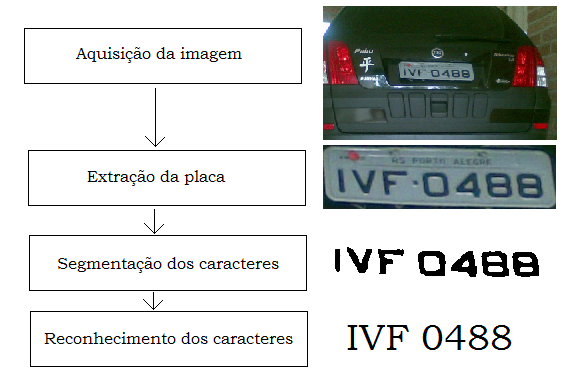
\includegraphics[width=88mm]{processo.png}
	\caption{Quatro estágios do reconhecimento de placa}
	\label{fig:processo}
\end{figure}

\section{Placa de Trânsito Brasileira}
\label{sec:placabr}

Segundo o código de trânsito brasileiro~\cite{brasil1997lei}, os veículos nacionais são identificados por meio de duas placas, dianteira e traseira, com exceção dos veículos de duas ou três rodas, que são dispensados da placa dianteira. As placas são identificadas por uma tarja na parte superior contendo a sigla do estado e o
nome do município, e pelo código de identificação único, composto por três
letras, seguidas por quatro dígitos, separados por um hífen.

Veículos particulares, de aluguel, oficial, de experiência, de aprendizagem e de
fabricante têm suas dimensões de \emph{130mmx400mm} e altura dos caracteres de 63mm (Figura~\ref{fig:placa_carro}).
Caso a placa não caiba no receptáculo ela pode ser reduzida em até 15\%. As
placas de motocicleta, motoneta, ciclomotor e triciclos autorizados têm
dimensões de \emph{136mmx187mm} e altura de caracteres de 42mm (Figura~\ref{fig:placa_moto}).

\begin{figure}[H]
	\centering
	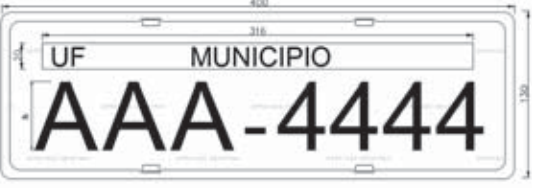
\includegraphics[width=88mm]{placa_carro.png}
	\caption{Placa de um carro}
	\label{fig:placa_carro}
\end{figure}

\begin{figure}[H]
	\centering
	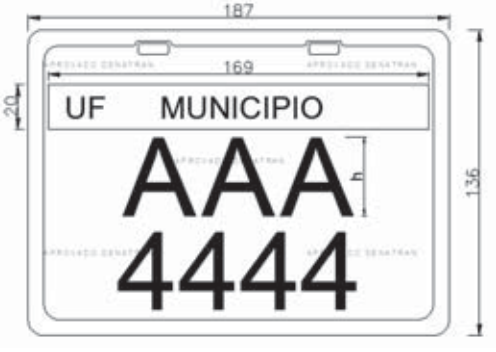
\includegraphics[width=88mm]{placa_moto.png}
	\caption{Placa de uma moto}
	\label{fig:placa_moto}
\end{figure}

A tipologia dos caracteres das placas utiliza a fonte \emph{Mandatory} (conforme mostra a Figura~\ref{fig:tipografia}), e as placas de categorias diferentes de veículos são diferenciadas pelas suas cores.

\begin{figure}[H]
	\centering
	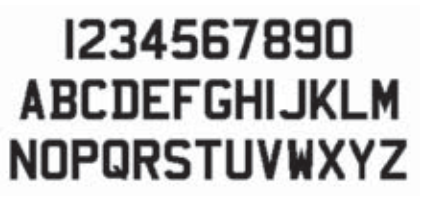
\includegraphics[width=88mm]{fonte.png}
	\caption{Tipografia das placas}
	\label{fig:tipografia}
\end{figure}

\section{Aquisição das imagens}
\label{sec:aquisicao}

O primeiro passo para o reconhecimento de uma placa é a extração das imagens. Diversos fatores externos podem afetar o reconhecimento da placa, como a iluminação, a distância e o ângulo da imagem. A escolha da posição onde as imagens serão adquiridas deve ser feita com o objetivo de minimizar esses problemas.

A aquisição das imagens será feita utilizando o módulo de câmera do
\emph{Raspberry Pi}. Trata-se uma câmera de 5 \emph{megapixels} capaz de gravar vídeos em 1080p, gerando imagens com dimensão de 1920×1080 \emph{pixels}. Uma das vantagens de utilizar essa combinação do \emph{Raspberry Pi} e seu módulo de câmera é a sua portabilidade. Por serem pequenos e leves, caso a câmera tenha dificuldade em capturar imagens que facilitam o reconhecimento das placas, é possível movê-los e colocá-los em posições privilegiadas para otimizar o processo.

\section{Extração da placa}
\label{sec:extracao}

A fase de extração é a fase mais importante em um sistema de reconhecimento de placas, porque todas as outras fases dependem da exata extração da área da placa. Essa extração é difícil pois influencia na precisão do sistema como um todo~\cite{kaur2014efficient}. Muitas dificuldades podem ocorrer durante a fase de extração pelos seguintes motivos:

\begin{itemize}
	\item A eficiência da extração é afetada pela complexidade da cena.
	\item Diferentes veículos possuem suas placas em diferentes posições.
	\item Pode ocorrer ruído durante a captura da câmera.
	\item Condições do tempo podem influenciar no ruído.
	\item Hora do dia afeta na luminosidade e resulta em erros de contraste.
	\item Outros caracteres, quadros e parafusos podem introduzir confusão.
	\item Mal posicionamento da câmera, ou placa, pode resultar em distorção que afeta na eficiência.
	\item Luminosidade baixa, ou desigual, imagem desfocada, baixa resolução, reflexão e sombra afetam a eficiência da extração.
\end{itemize}

O método implementado é baseado em Kaur~\cite{kaur2014efficient} e segue o seguinte fluxograma:

\begin{enumerate}
	\item Conversão de RGB para escala de tons de cinza.
	\item Remoção de ruído por filtro bilateral.
	\item Aumento de contraste usando equalização de histograma adaptativo.
	\item Binarização da Imagem.
	\item Detecção de borda pelo operador \emph{Sobel}.
    \item Operação de dilatação sobre as bordas.
    \item Preenchimento de buracos na imagem.
	\item Detecção de área de placa candidata por operações morfológicas de abertura e fechamento.
	\item Extração da área da placa real.
    \item Aprimoramento da região extraída.
\end{enumerate}

\subsection{Conversão de RGB para escala de tons de cinza}

A imagem capturada está no formato RGB\@. O primeiro passo do pré-processamento é converter essa imagem para a escala de tons de cinza. O objetivo dessa conversão é reduzir o número de cores. Os componentes R, G e B são separados do valor de cor de 24 bits de cada pixel (i,j), e um valor de 8 bits em cinza é calculado. Uma imagem capturada e convertida para tons de cinza pode ser vista na Figura~\ref{fig:ext_gray_scale}.

\begin{figure}[H]
	\centering
	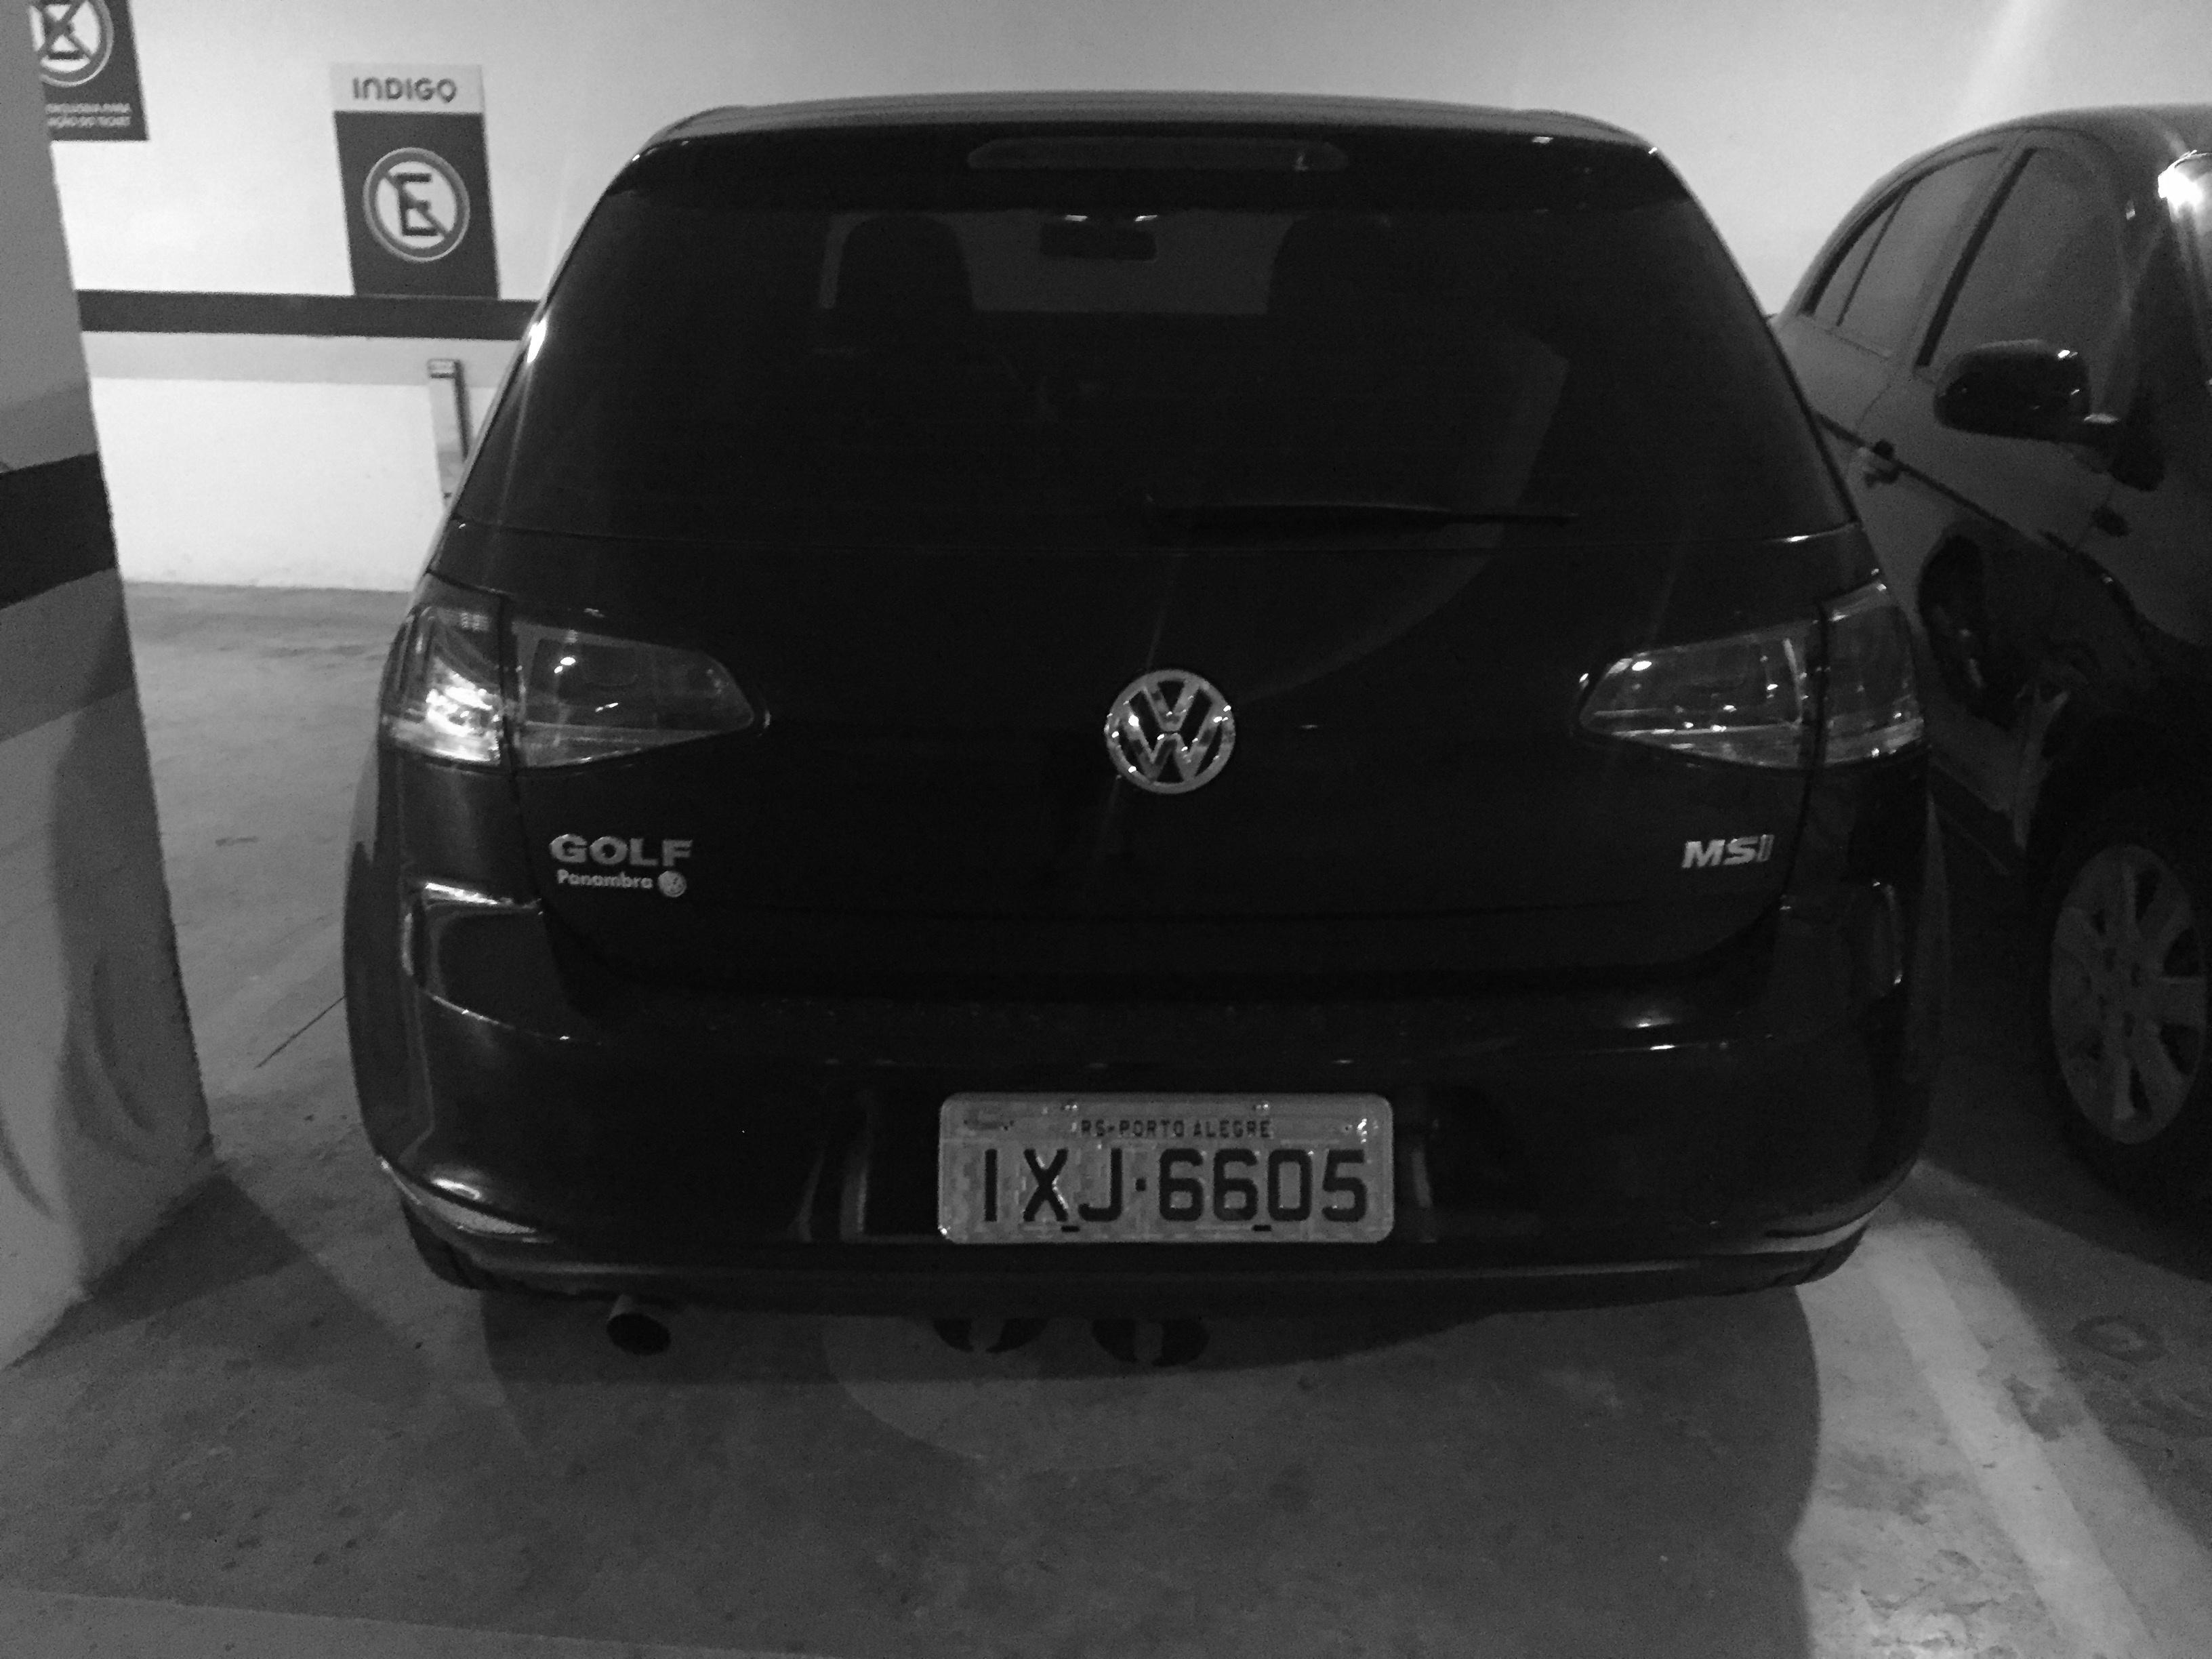
\includegraphics[width=88mm]{1grayscale.jpg}
	\caption{Imagem em escala de tons de cinza.}
	\label{fig:ext_gray_scale}
\end{figure}

\subsection{Remoção de ruído por filtro bilateral}

O filtro bilateral é um filtro não linear, que preserva as arestas e reduz ruído. Ele funciona substituindo o valor de intensidade de cada \emph{pixel} em uma imagem por uma média ponderada dos valores de intensidade dos \emph{pixels} próximos. O objetivo básico da filtragem é remover ruído e distorção da imagem. O ruído pode ocorrer durante a captura pela câmera ou pelas condições do tempo. No método que Kaur~\cite{kaur2014efficient} propõe, o filtro bilateral iterativo é utilizado para remover ruído. Ele é não linear, provê mecanismo para remoção de ruído enquanto preserva bordas mais efetivamente que o filtro mediano. O filtro mediano funciona substituindo o valor de cada \emph{pixel} pela mediana dos \emph{pixels} vizinhos. Na Figura~\ref{fig:ext_filter_in_gray_scale} pode-se ver a imagem em tons de cinza com a remoção de ruído por filtro bilateral aplicada.

\begin{figure}[H]
	\centering
	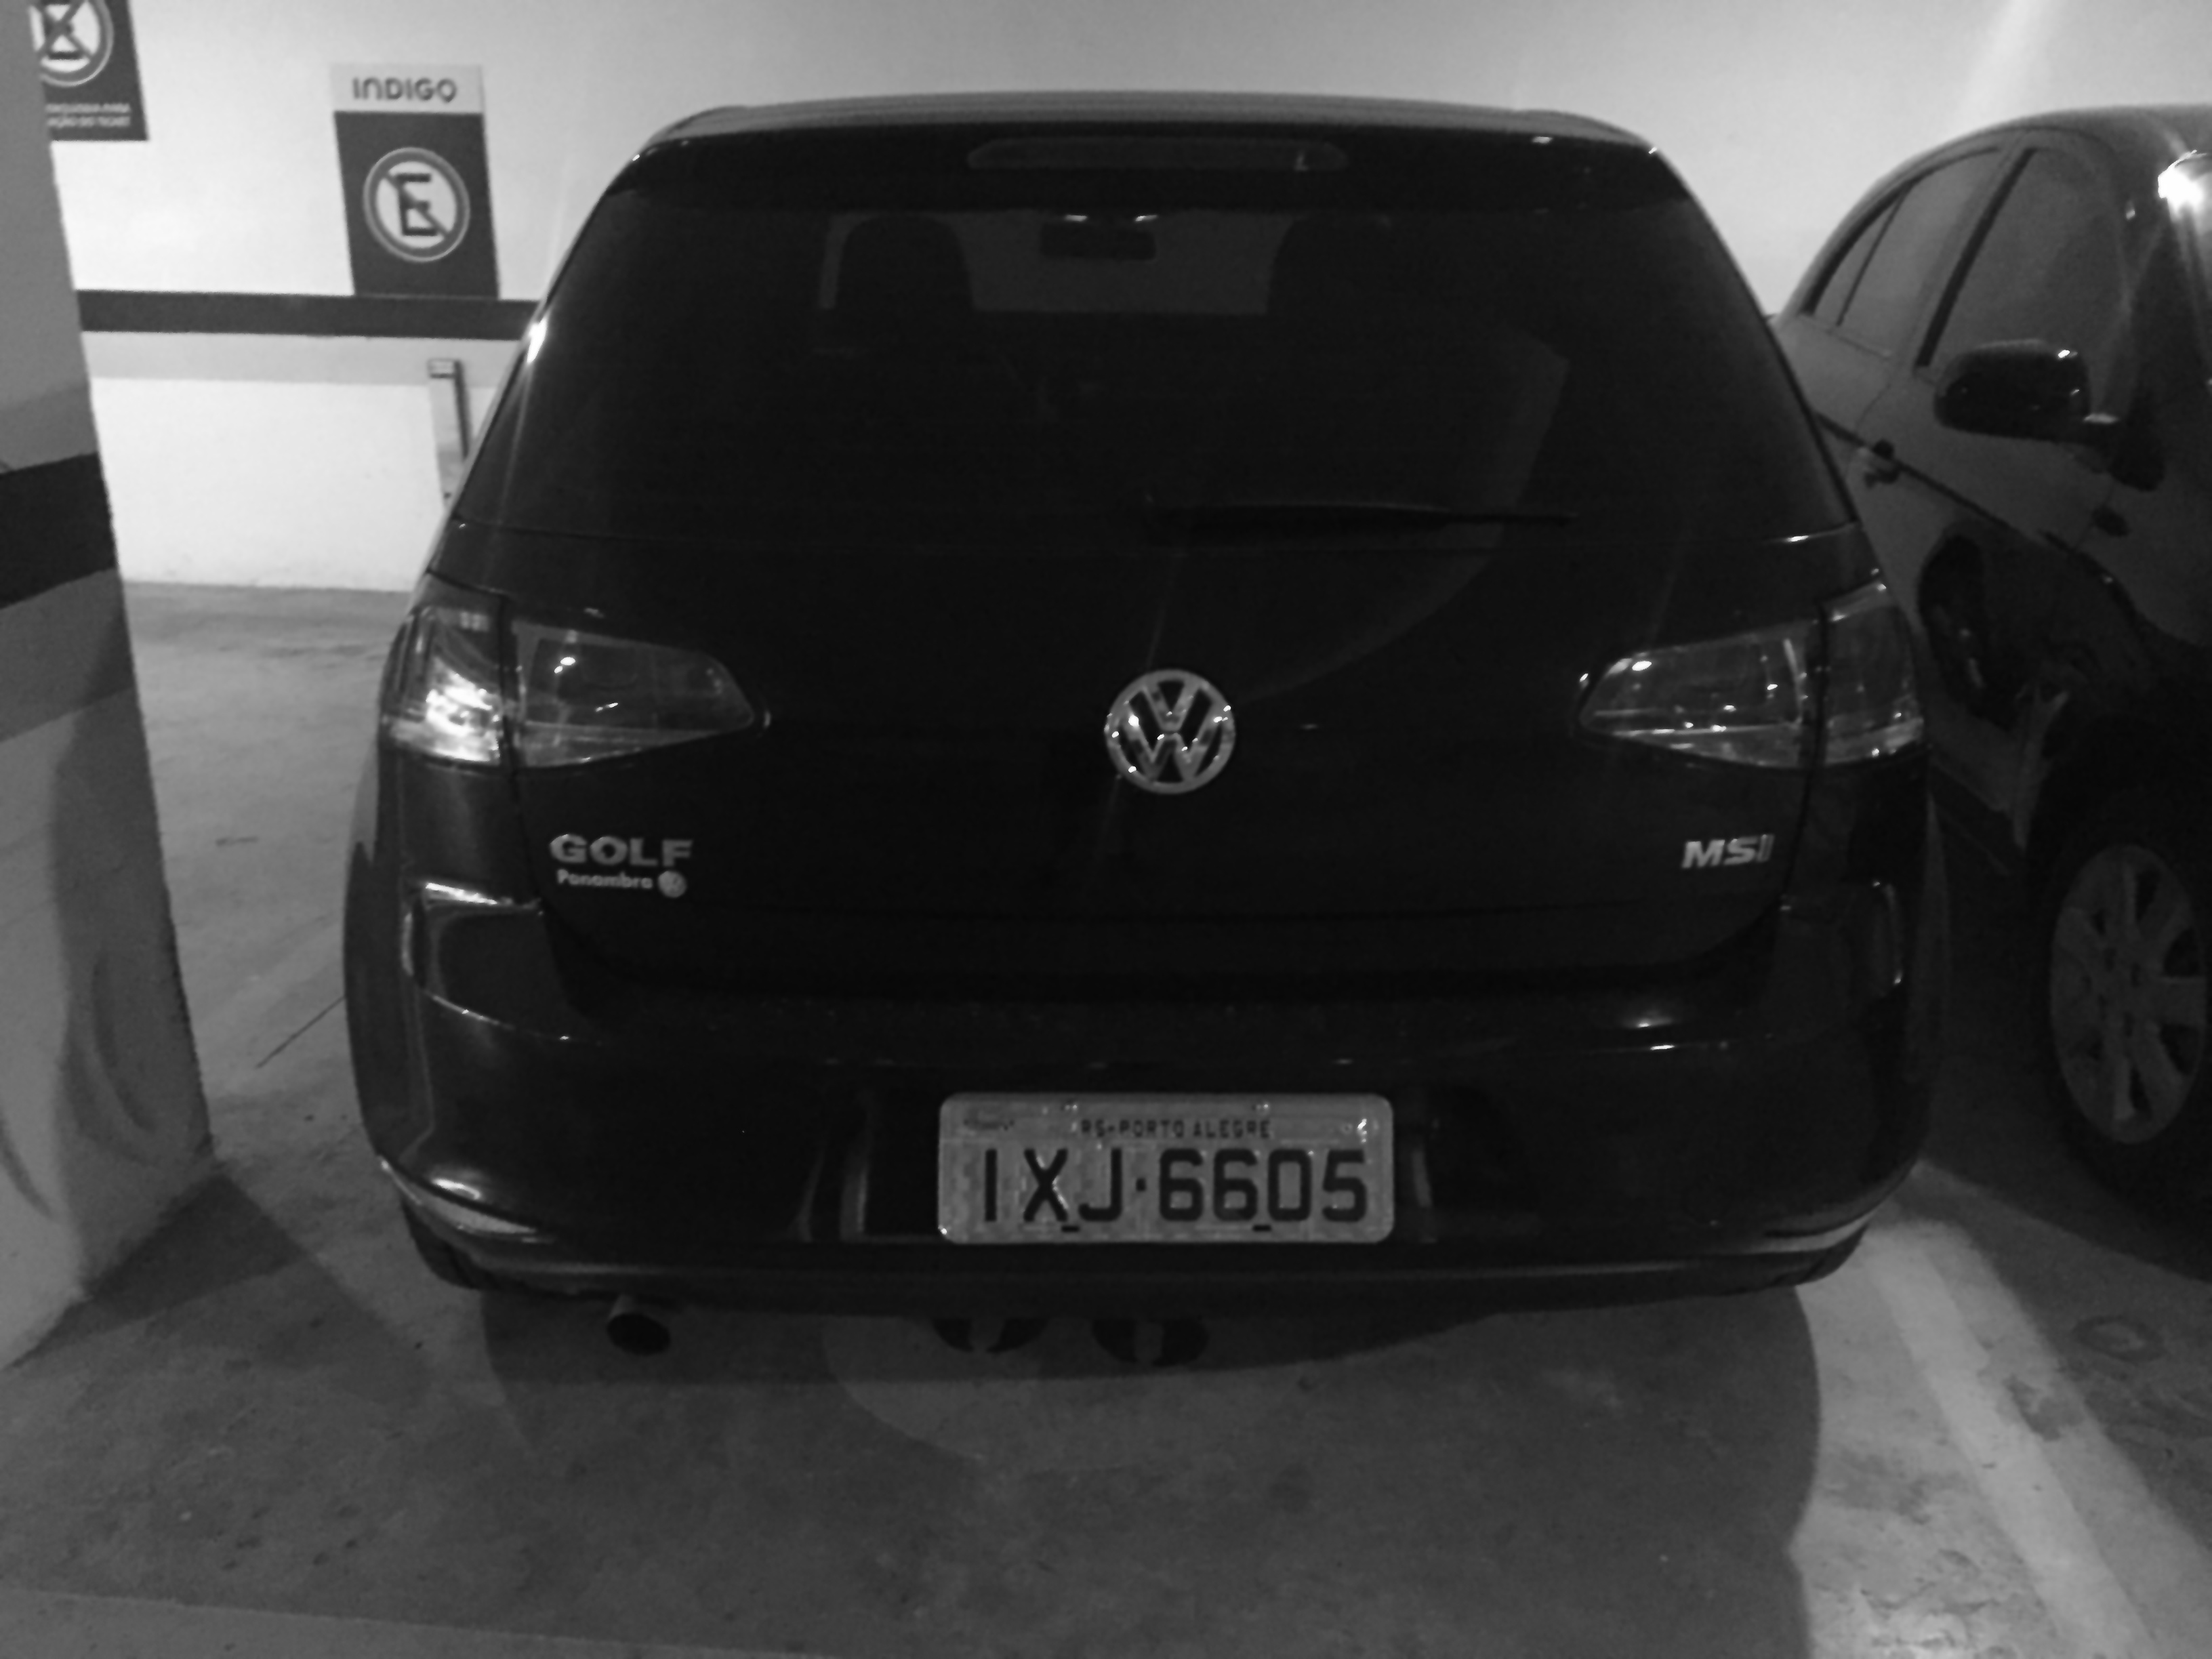
\includegraphics[width=88mm]{2bilateral.jpg}
	\caption{Aplicação de filtro bilateral em uma imagem em escala de tons de cinza}
	\label{fig:ext_filter_in_gray_scale}
\end{figure}

É necessário utilizar um filtro de remoção de ruído que tenha capacidade de preservar as bordas, pois a detecção de bordas é um passo muito importante na extração da placa. A detecção de bordas será abordada na Seção~\ref{sec:detec_bordas}. 

\subsection{Aumento de contraste usando equalização de histograma adaptativo}

Contraste é definido como a diferença entre o nível mais baixo e alto de
intensidade. Equalização de histograma é o método para distribuir de forma mais efetiva o histograma de \emph{pixels}. Equalização de histograma adaptativo mostra melhor contraste em relação a equalização de histograma. Na Figura~\ref{fig:ext_contrast_adaptive_histogram} foi aplicado o aumento de contraste utilizando equalização de histograma adaptativo sobre a imagem anterior (Figura~\ref{fig:ext_filter_in_gray_scale}).

\begin{figure}[H]
	\centering
	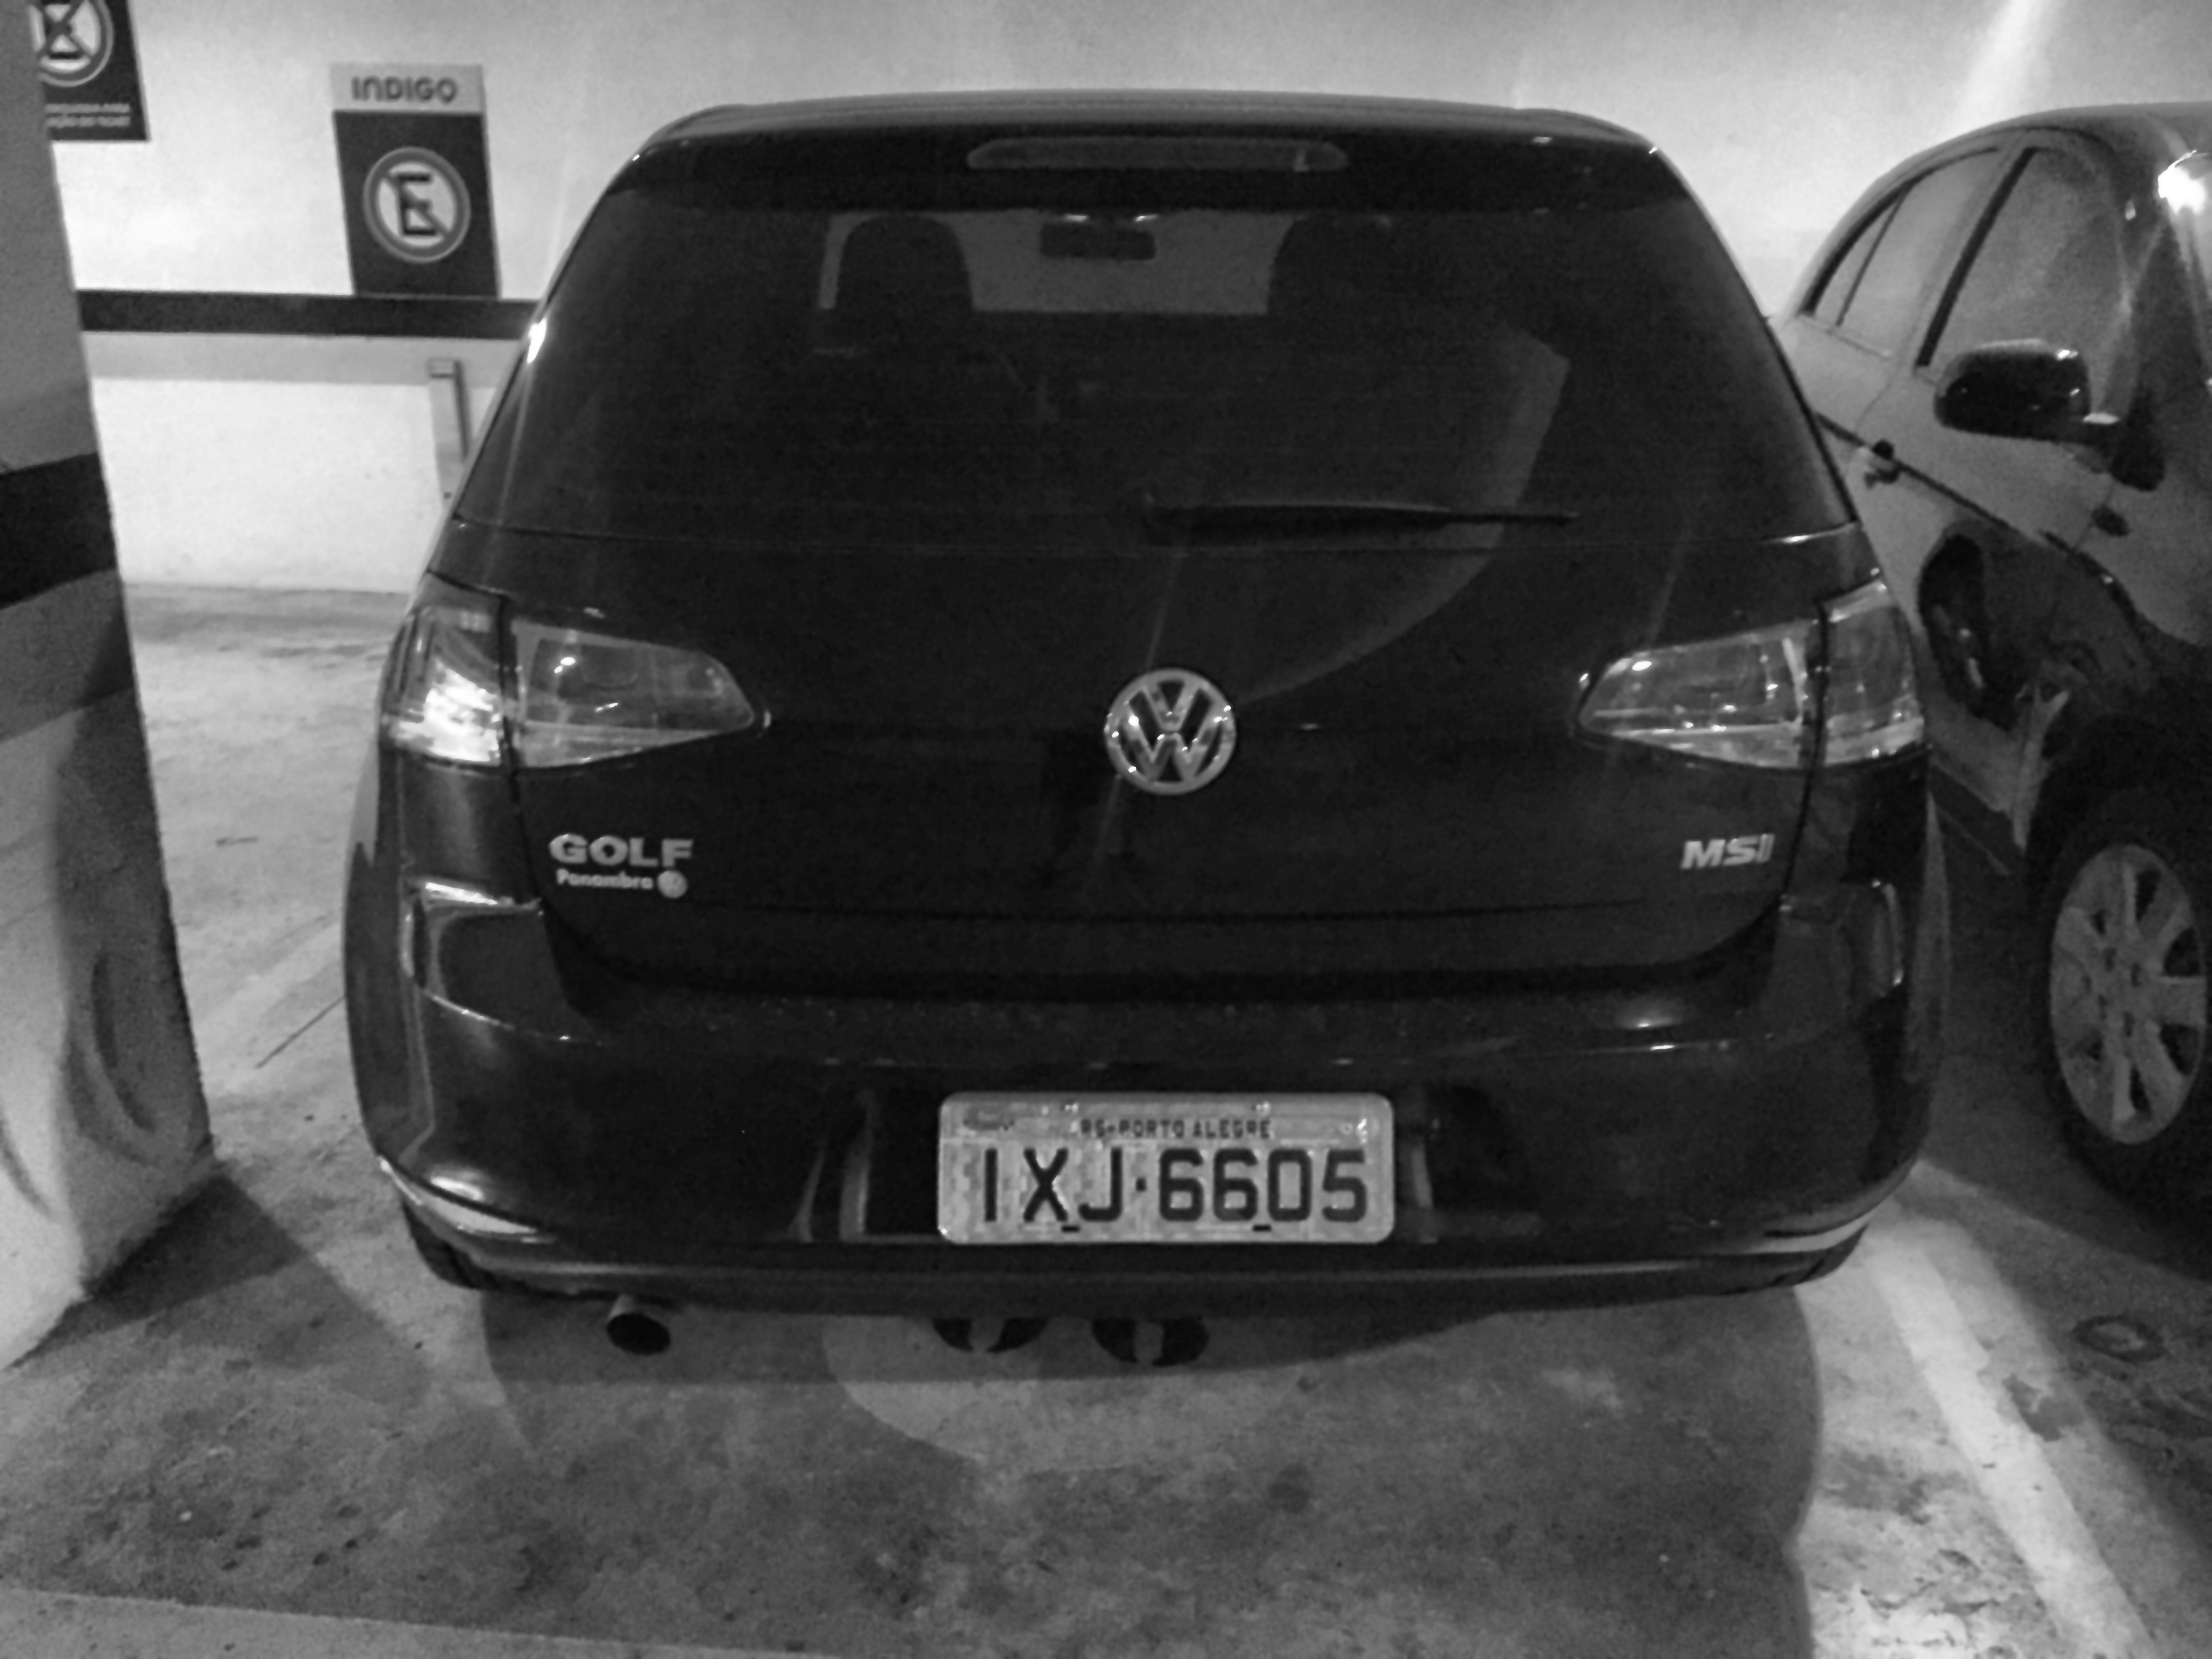
\includegraphics[width=88mm]{3histogram_eq.jpg}
	\caption{Aumento de contraste usando equalização de histograma adaptativo}
	\label{fig:ext_contrast_adaptive_histogram}
\end{figure}

\subsection{Binarização da Imagem}

Nesta operação a imagem de escala de cinza pré-processada é convertida em imagem binária. Para isso é utilizada uma técnica de limiarização. Na implementação de Kaur~\cite{kaur2014efficient}, foi escolhida uma técnica de limiarização por limiar global, utilizando o método de \emph{Otsu} para calcular esse limiar. 

O algoritmo do método de \emph{Otsu} assume que  a imagem contém duas classes de \emph{pixels} seguindo um histograma bi-modal. Ele calcula o limiar ótimo separando as duas classes para que o seu espalhamento combinado seja mínimo. Tendo o limiar calculado, a imagem de escala de cinza subtraída é convertida em imagem em preto e branco.

O objetivo final desse passo, é fazer com que, na imagem binarizada, haja uma diferença entre a cor da placa e a cor do resto do carro, deixando a placa demarcada na imagem. O resultado dessa binarização pode ser visto na Figura~\ref{fig:ext_binarized_image}.

\begin{figure}[H]
	\centering
	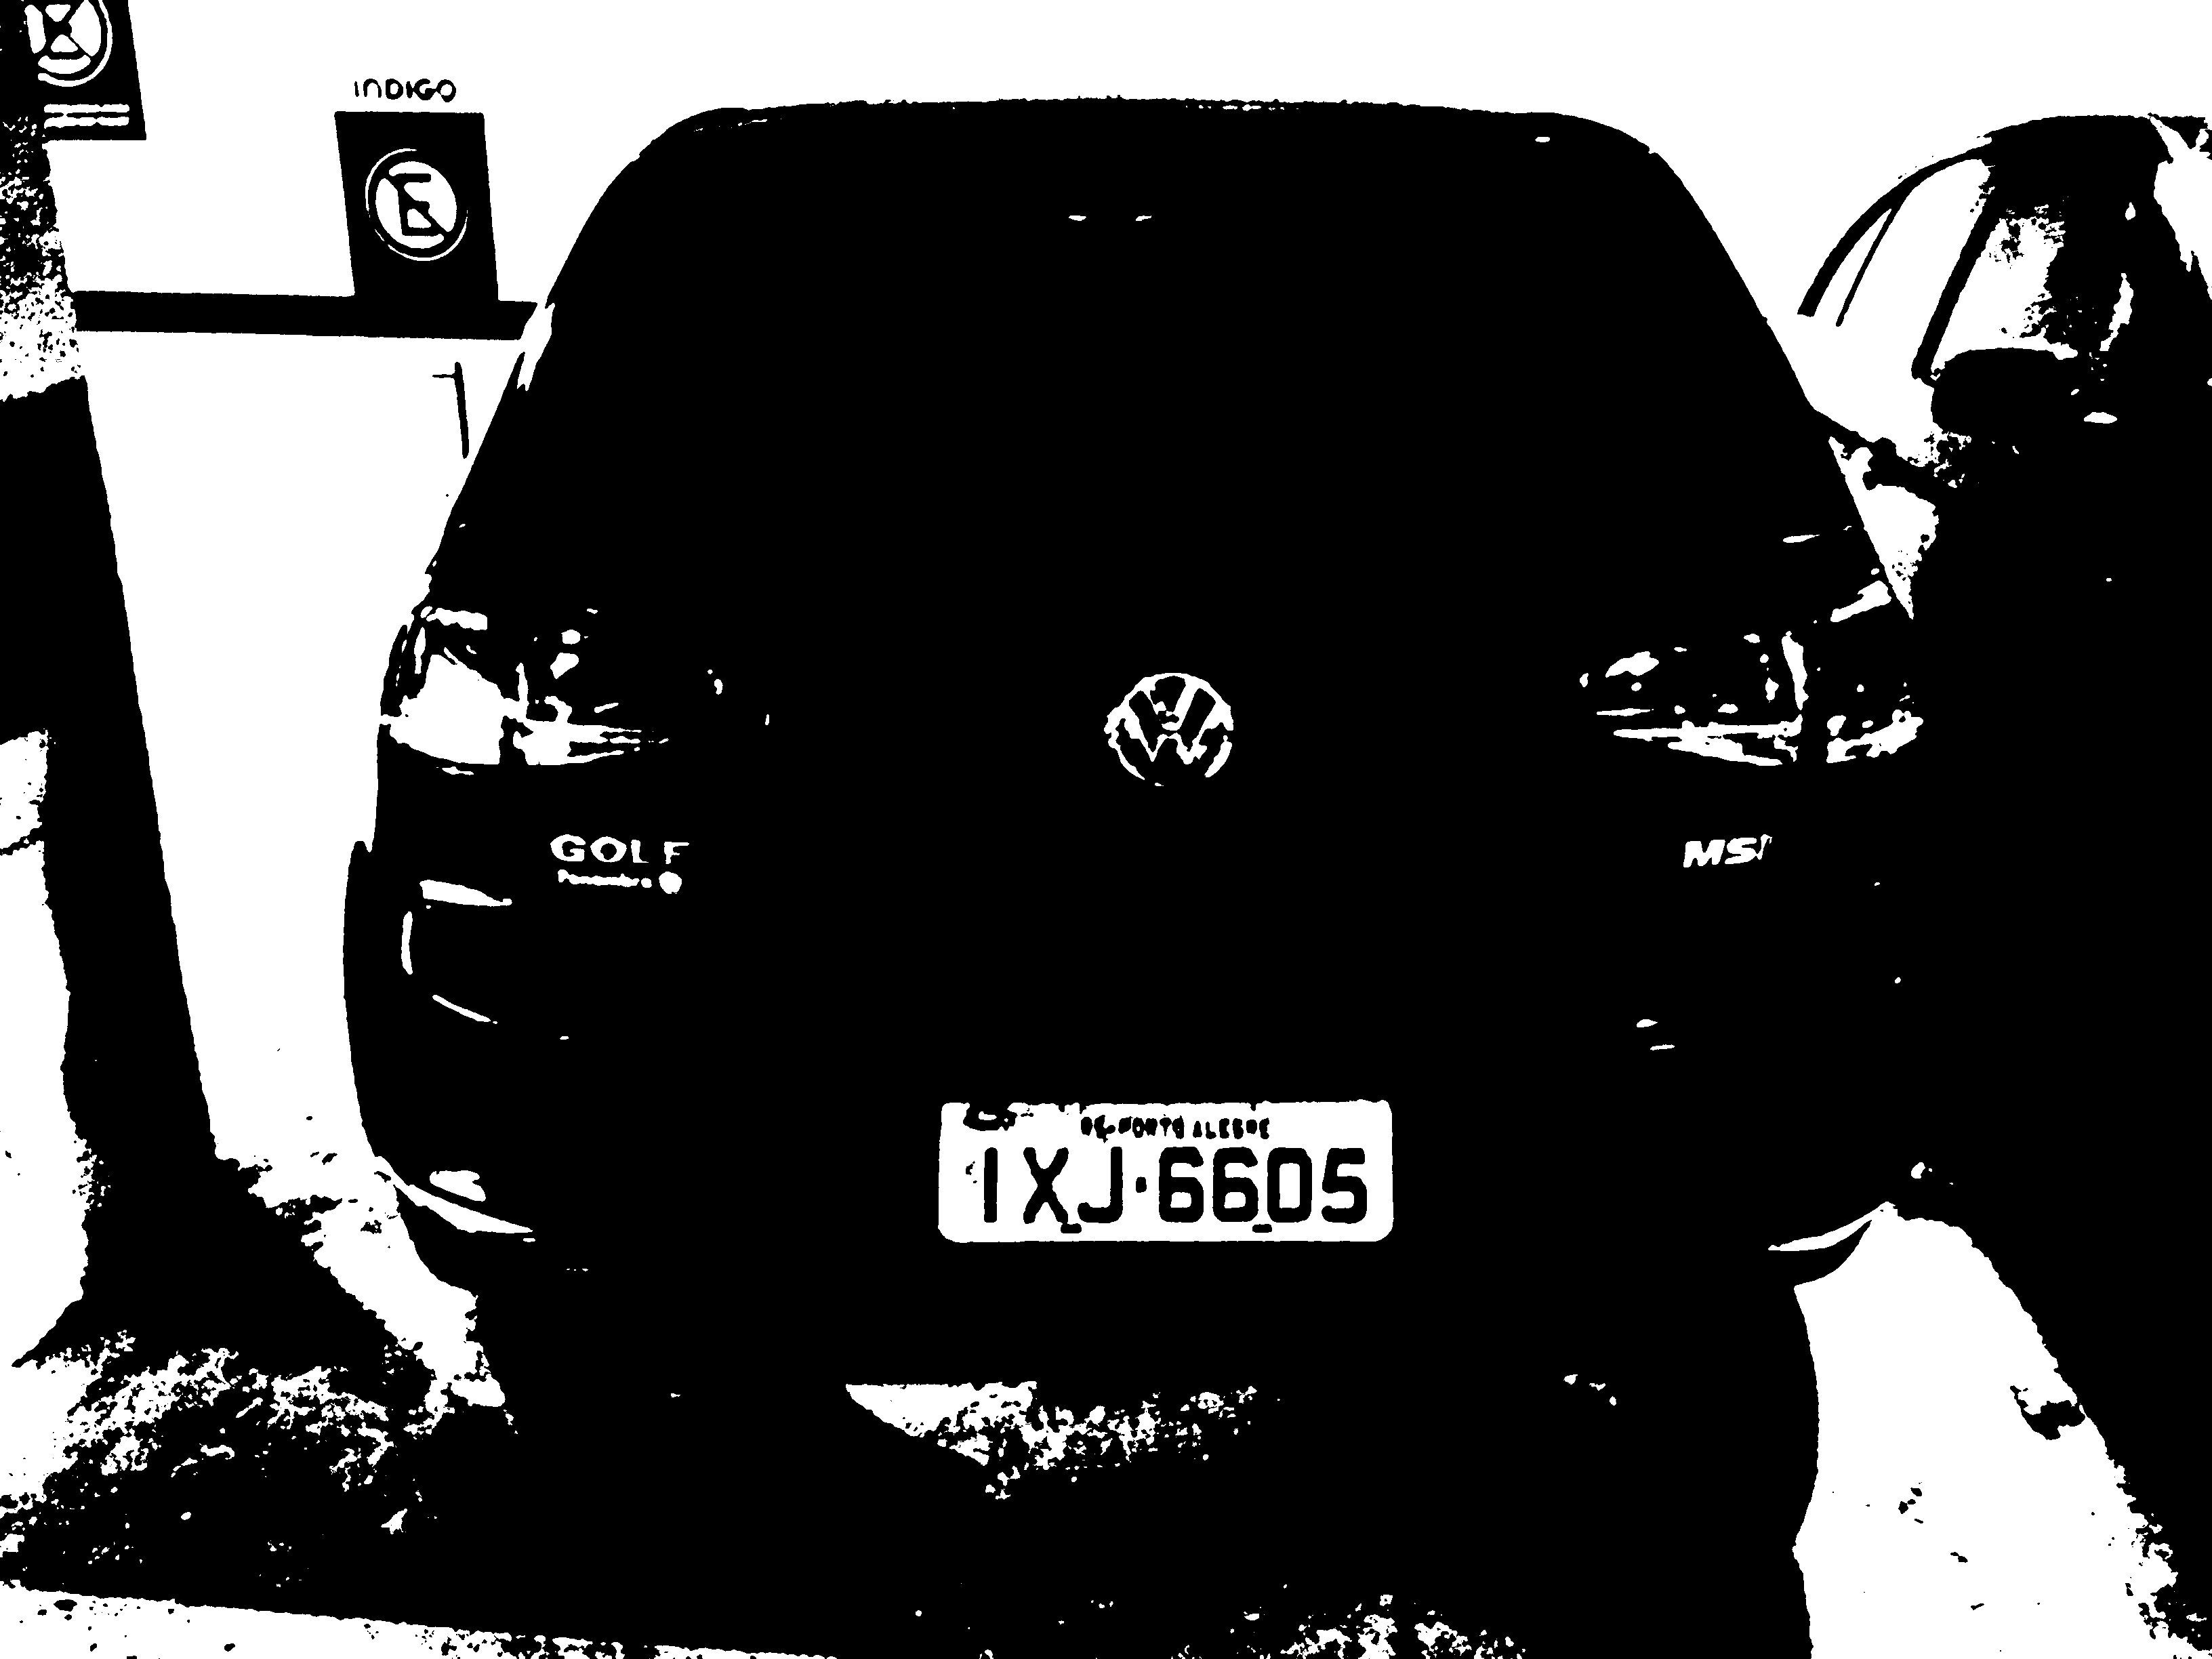
\includegraphics[width=88mm]{4binarized_image.jpg}
	\caption{Imagem Binarizada}
	\label{fig:ext_binarized_image}
\end{figure}

\subsection{Detecção de borda pelo operador Sobel}
\label{sec:detec_bordas}

Neste passo as bordas da imagem são detectadas pelo operador de \emph{Sobel}. A detecção de bordas em uma imagem diminui significantemente a quantidade de dados a ser processados e remove informações desnecessárias, enquanto preserva importantes propriedades estruturais na imagem~\cite{ha2016license}.

Para que esse passo tenha sucesso, é necessário que, na binarização, a placa e o resto do carro tenham obtido valores diferentes. Com isso, a detecção de bordas terá como objetivo desenhar o contorno da placa do carro, incluindo, ou não, outros elementos não relevantes da imagem. O resultado da detecção de bordas aplicada à imagem binarizada é mostrado na Figura~\ref{fig:ext_edge_detection_sobel}.

\begin{figure}[H]
	\centering
	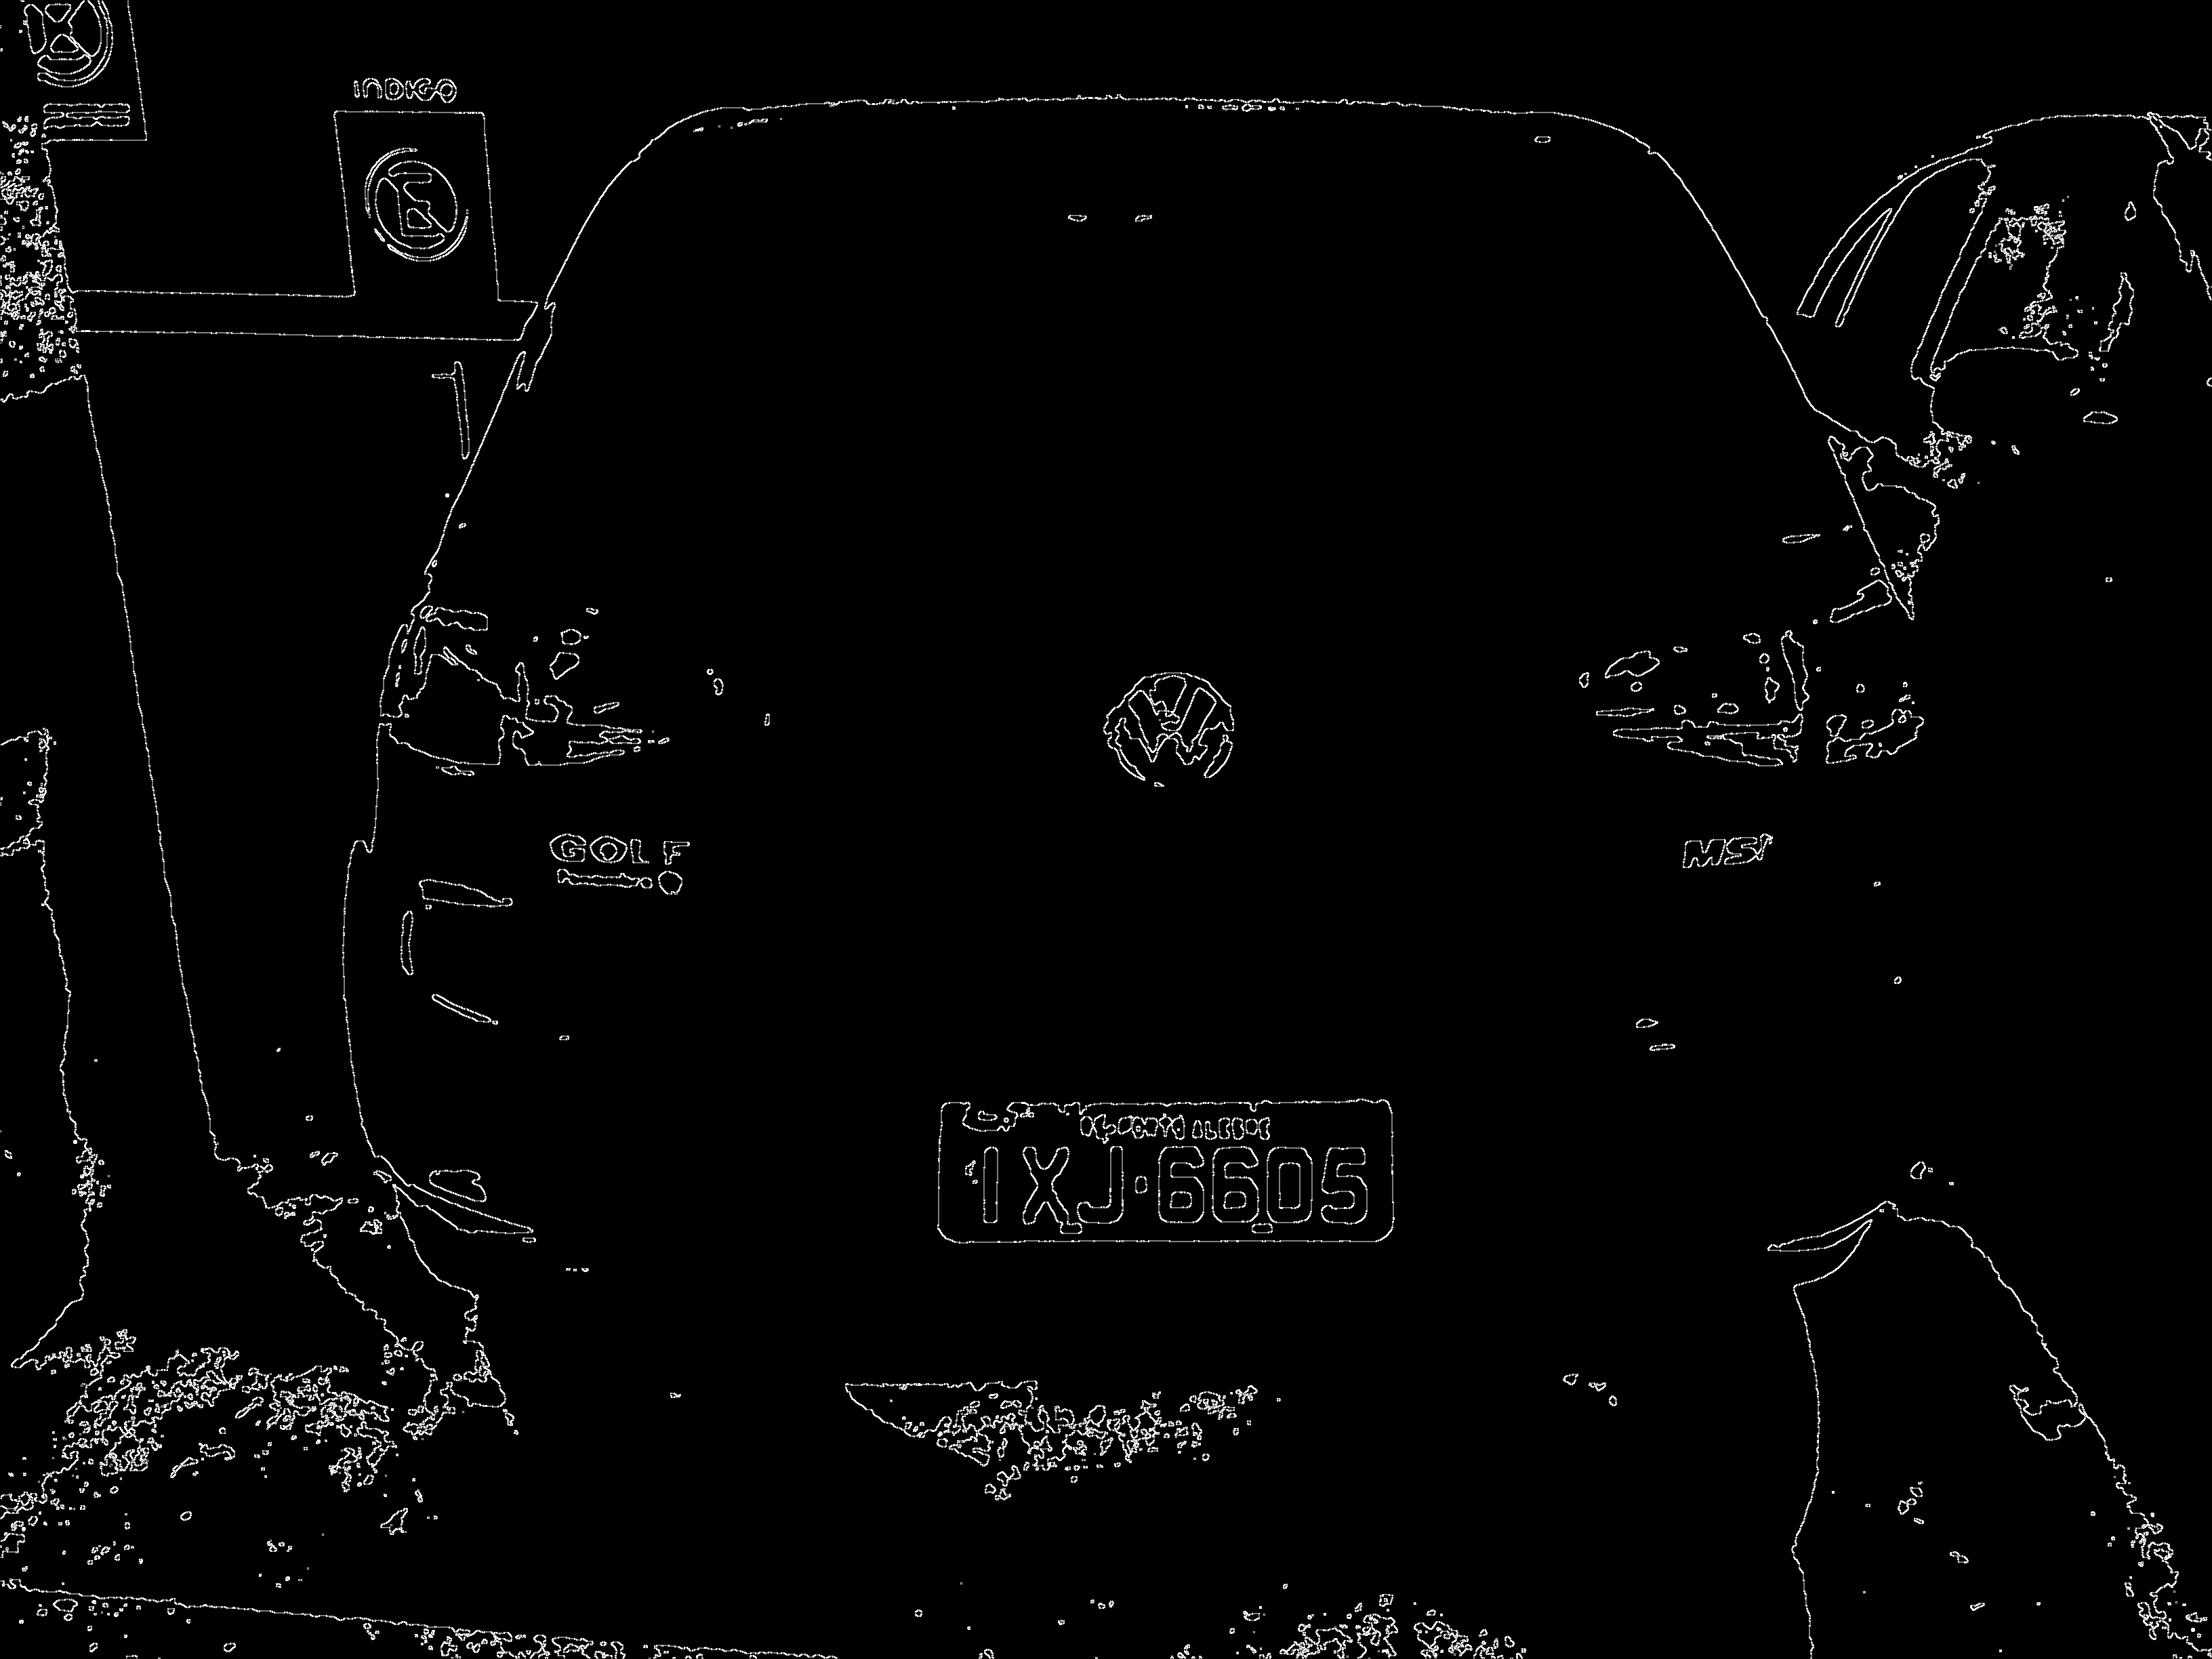
\includegraphics[width=88mm]{5sobel_image.jpg}
	\caption{Detecção de borda pelo operador Sobel}
	\label{fig:ext_edge_detection_sobel}
\end{figure}

\subsection{Operação de dilatação sobre as bordas}

Tendo as bordas detectadas deve-se aplicar uma operação de dilatação sobre a imagem processada. O motivo deste passo é deixar as bordas detectadas mais fortes. Na operação anterior é possível que existam pequenos furos nas bordas geradas, segmentando a linha desenhada em diversos pedaços. Aplicando a dilatação sobre essas bordas, as linhas se fecham deixando as bordas mais definidas.

As bordas precisam ser bem definidas para garantir que o retângulo gerado pela placa esteja completo. Espaços abertos nessa área podem causar complicações nas etapas seguintes. Na Figura~\ref{fig:ext_morphological_dilation} é possível ver as bordas dilatadas e mais definidas.

\begin{figure}[H]
	\centering
	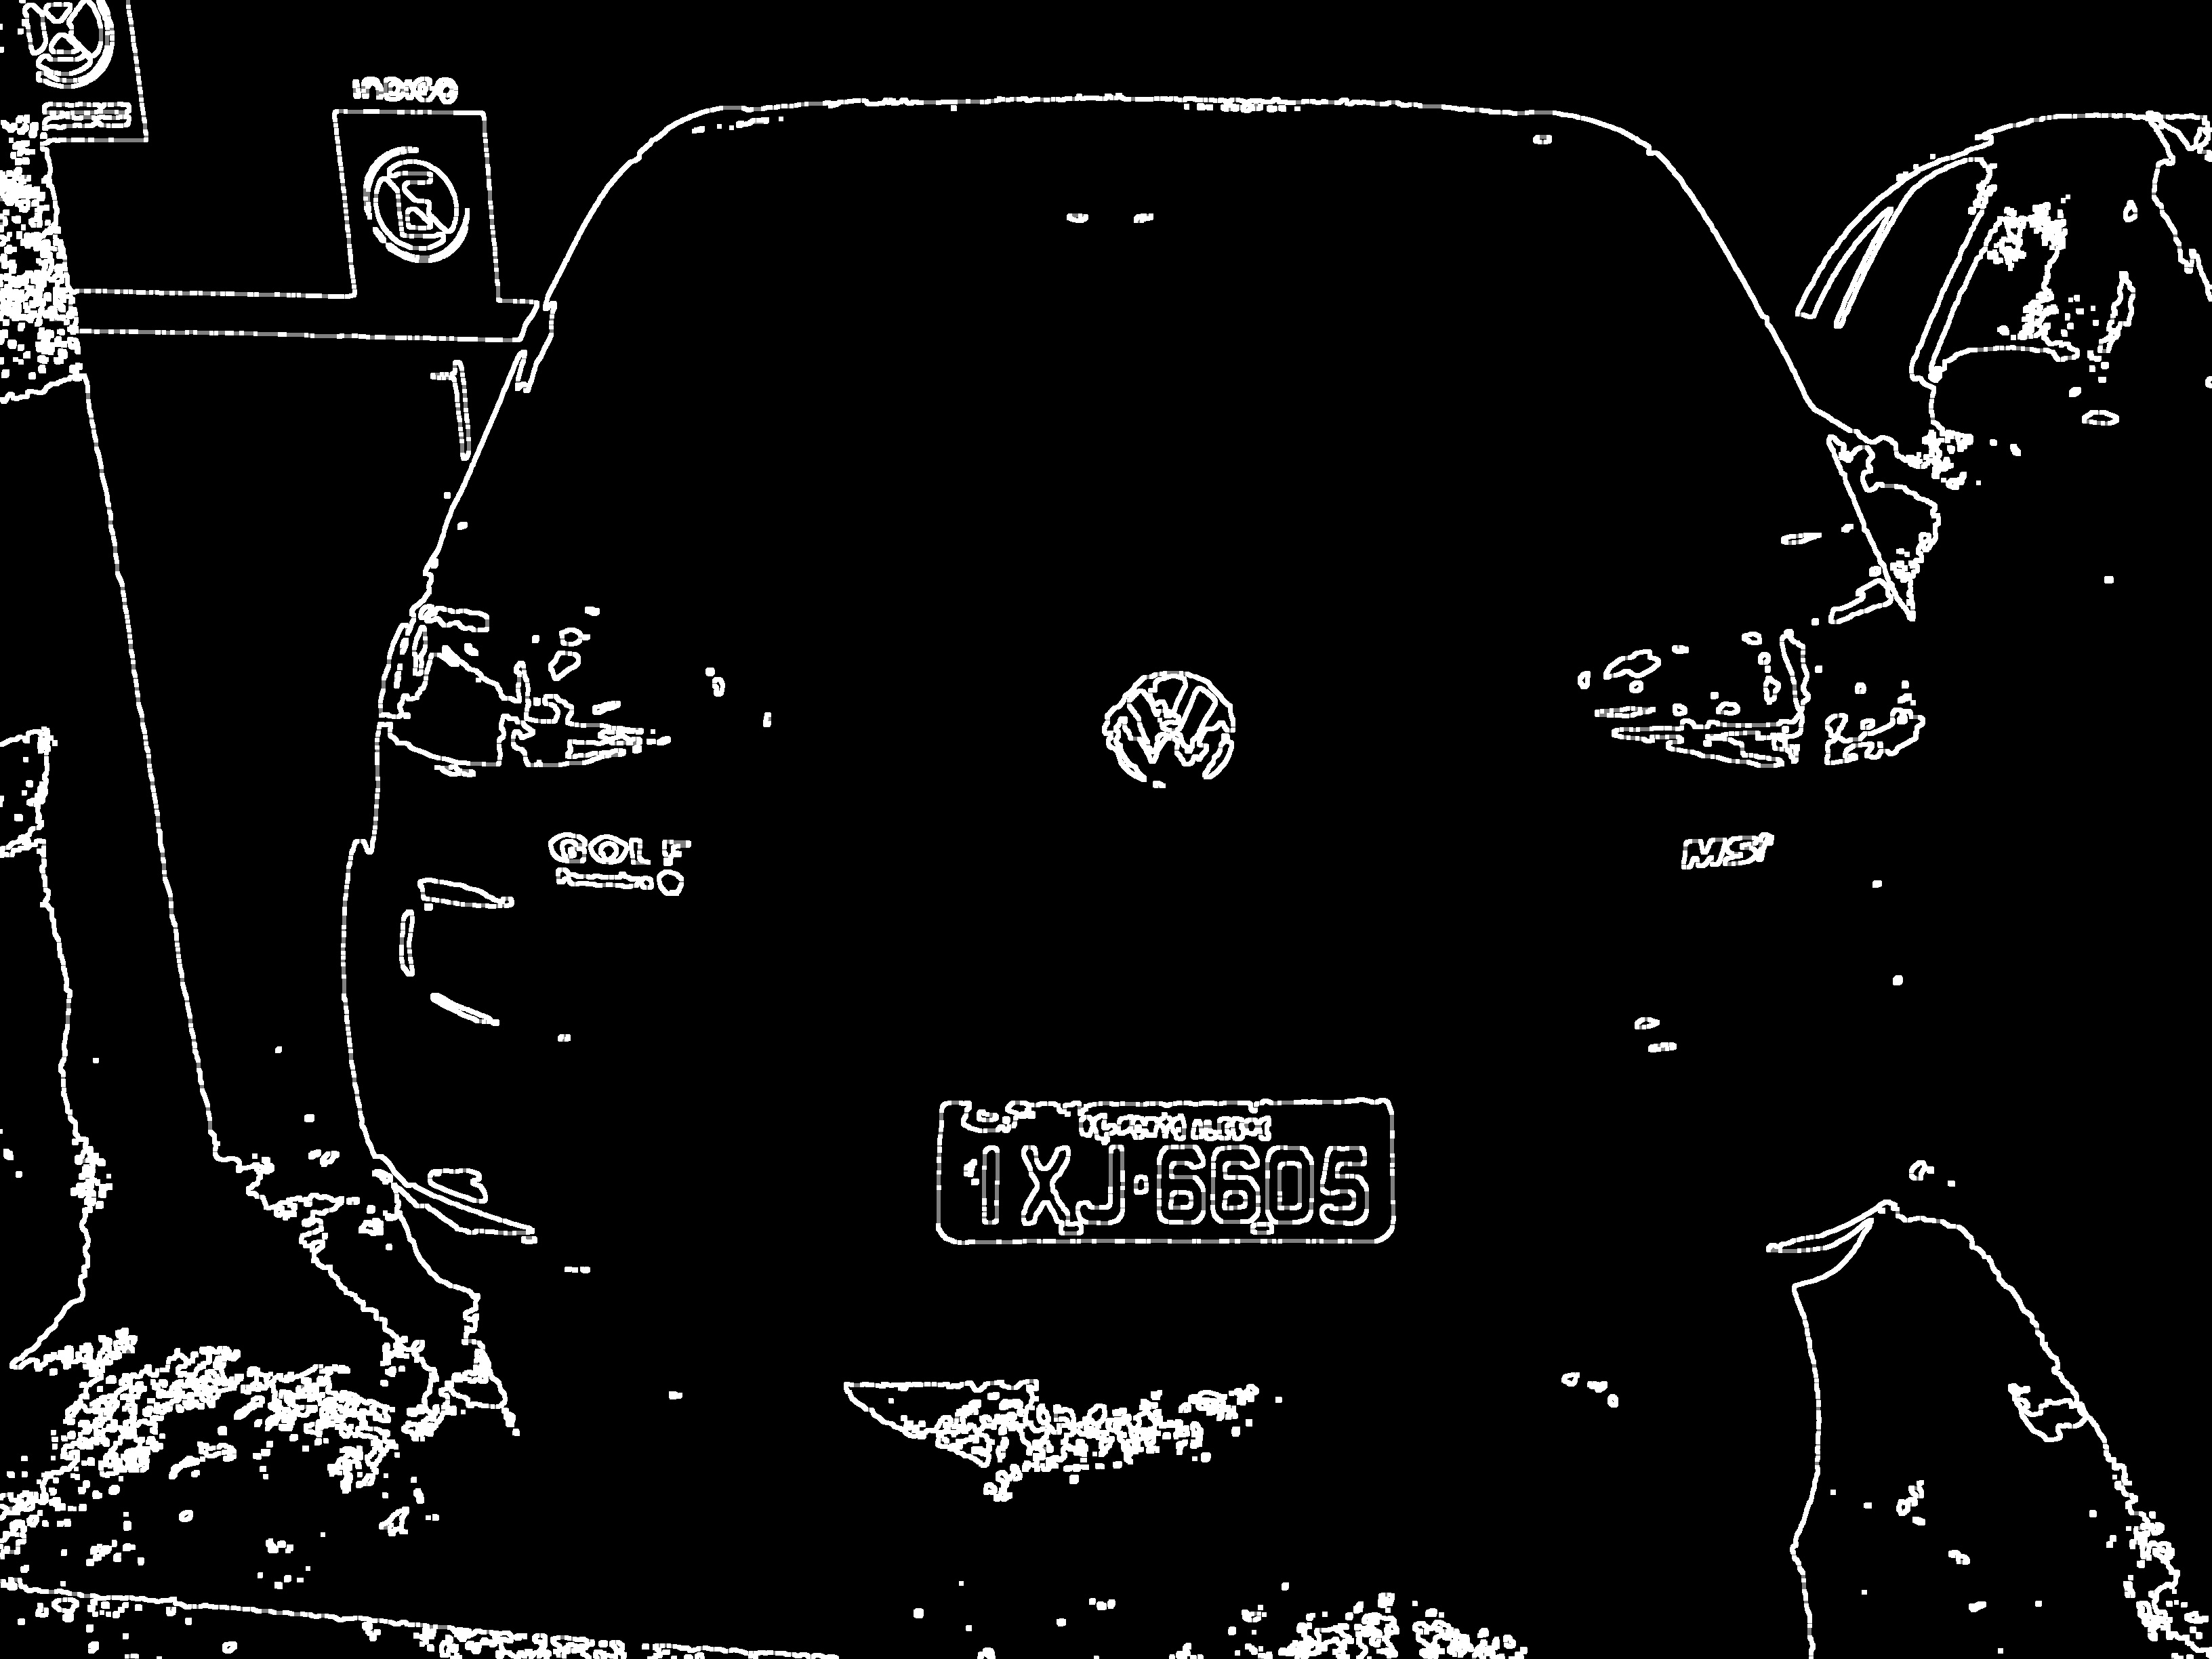
\includegraphics[width=88mm]{6dilated_image.jpg}
	\caption{Dilatação morfológica}
	\label{fig:ext_morphological_dilation}
\end{figure}

\subsection{Preenchimento de buracos na imagem}

Com as bordas dilatadas e bem definidas é feito o preenchimento das áreas fechadas na imagem. Se as bordas ao redor da placa estiverem corretamente demarcadas, nesta etapa, sobre a área da placa, haverá um retângulo completo fechado. Essa é a etapa da detecção das áreas de placa onde é possível identificar visualmente os candidatos a placa. Estes são os pontos onde existem grandes conjuntos de \emph{pixels}, as áreas com bordas fechadas que foram preenchidas. Na Figura~\ref{fig:ext_holes_filled} pode-se ver a imagem com os buracos preenchidos.

\begin{figure}[H]
	\centering
	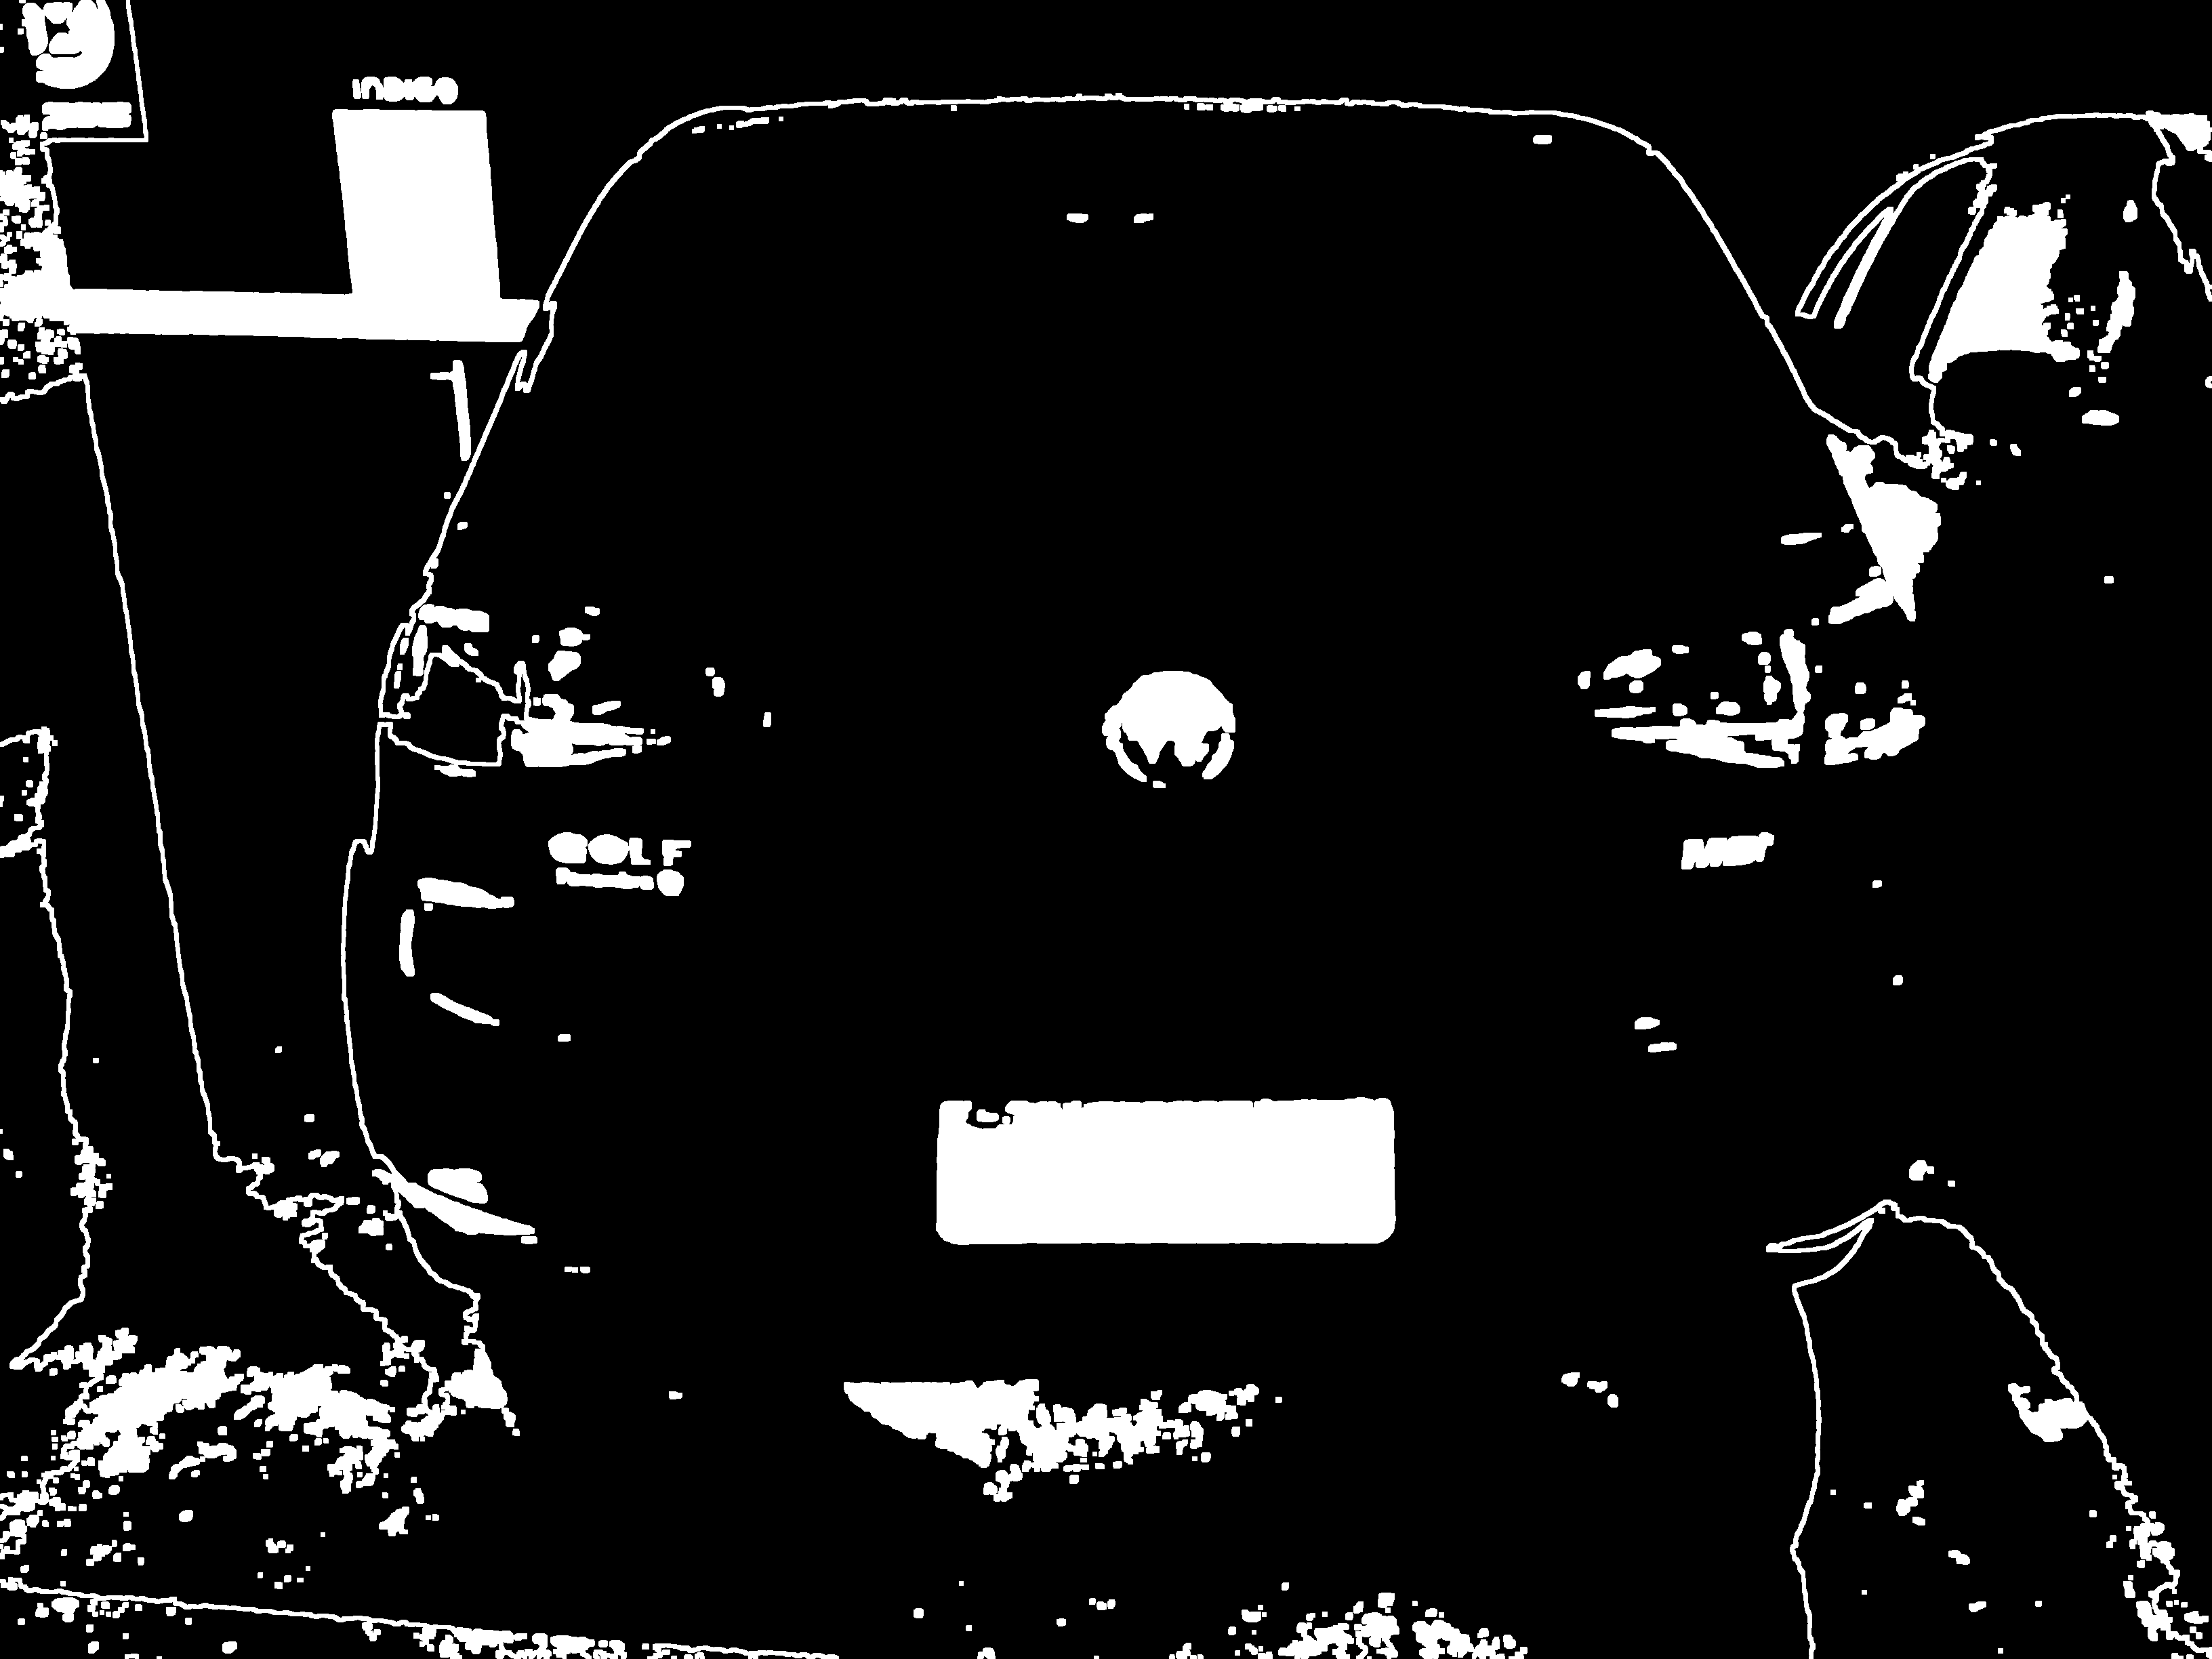
\includegraphics[width=88mm]{7filled_image.png}
	\caption{Após preenchimento dos buracos}
	\label{fig:ext_holes_filled}
\end{figure}

\subsection{Detecção de Áreas de Placa Candidatas por Operações Morfológicas de Abertura e Fechamento}

Com as operações morfológicas, os objetos indesejados na imagem são removidos. As operações de abertura e fechamento são usadas para a detecção exata da área da placa. Essa etapa acaba se tornando um pouco limitada, pois o elemento estruturante deve ser de certa forma proporcional ao tamanho da placa na imagem. Com um elemento estruturante muito pequeno, sobram muitos candidatos falsos, pois eles não são removidos nas operações morfológicas. Com um elemento estruturante muito grande, a área da placa pode ser removida junto com o ruído. A Figura~\ref{fig:ext_plate_area_detection} contém as regiões candidatas da placa.

\begin{figure}[H]
	\centering
	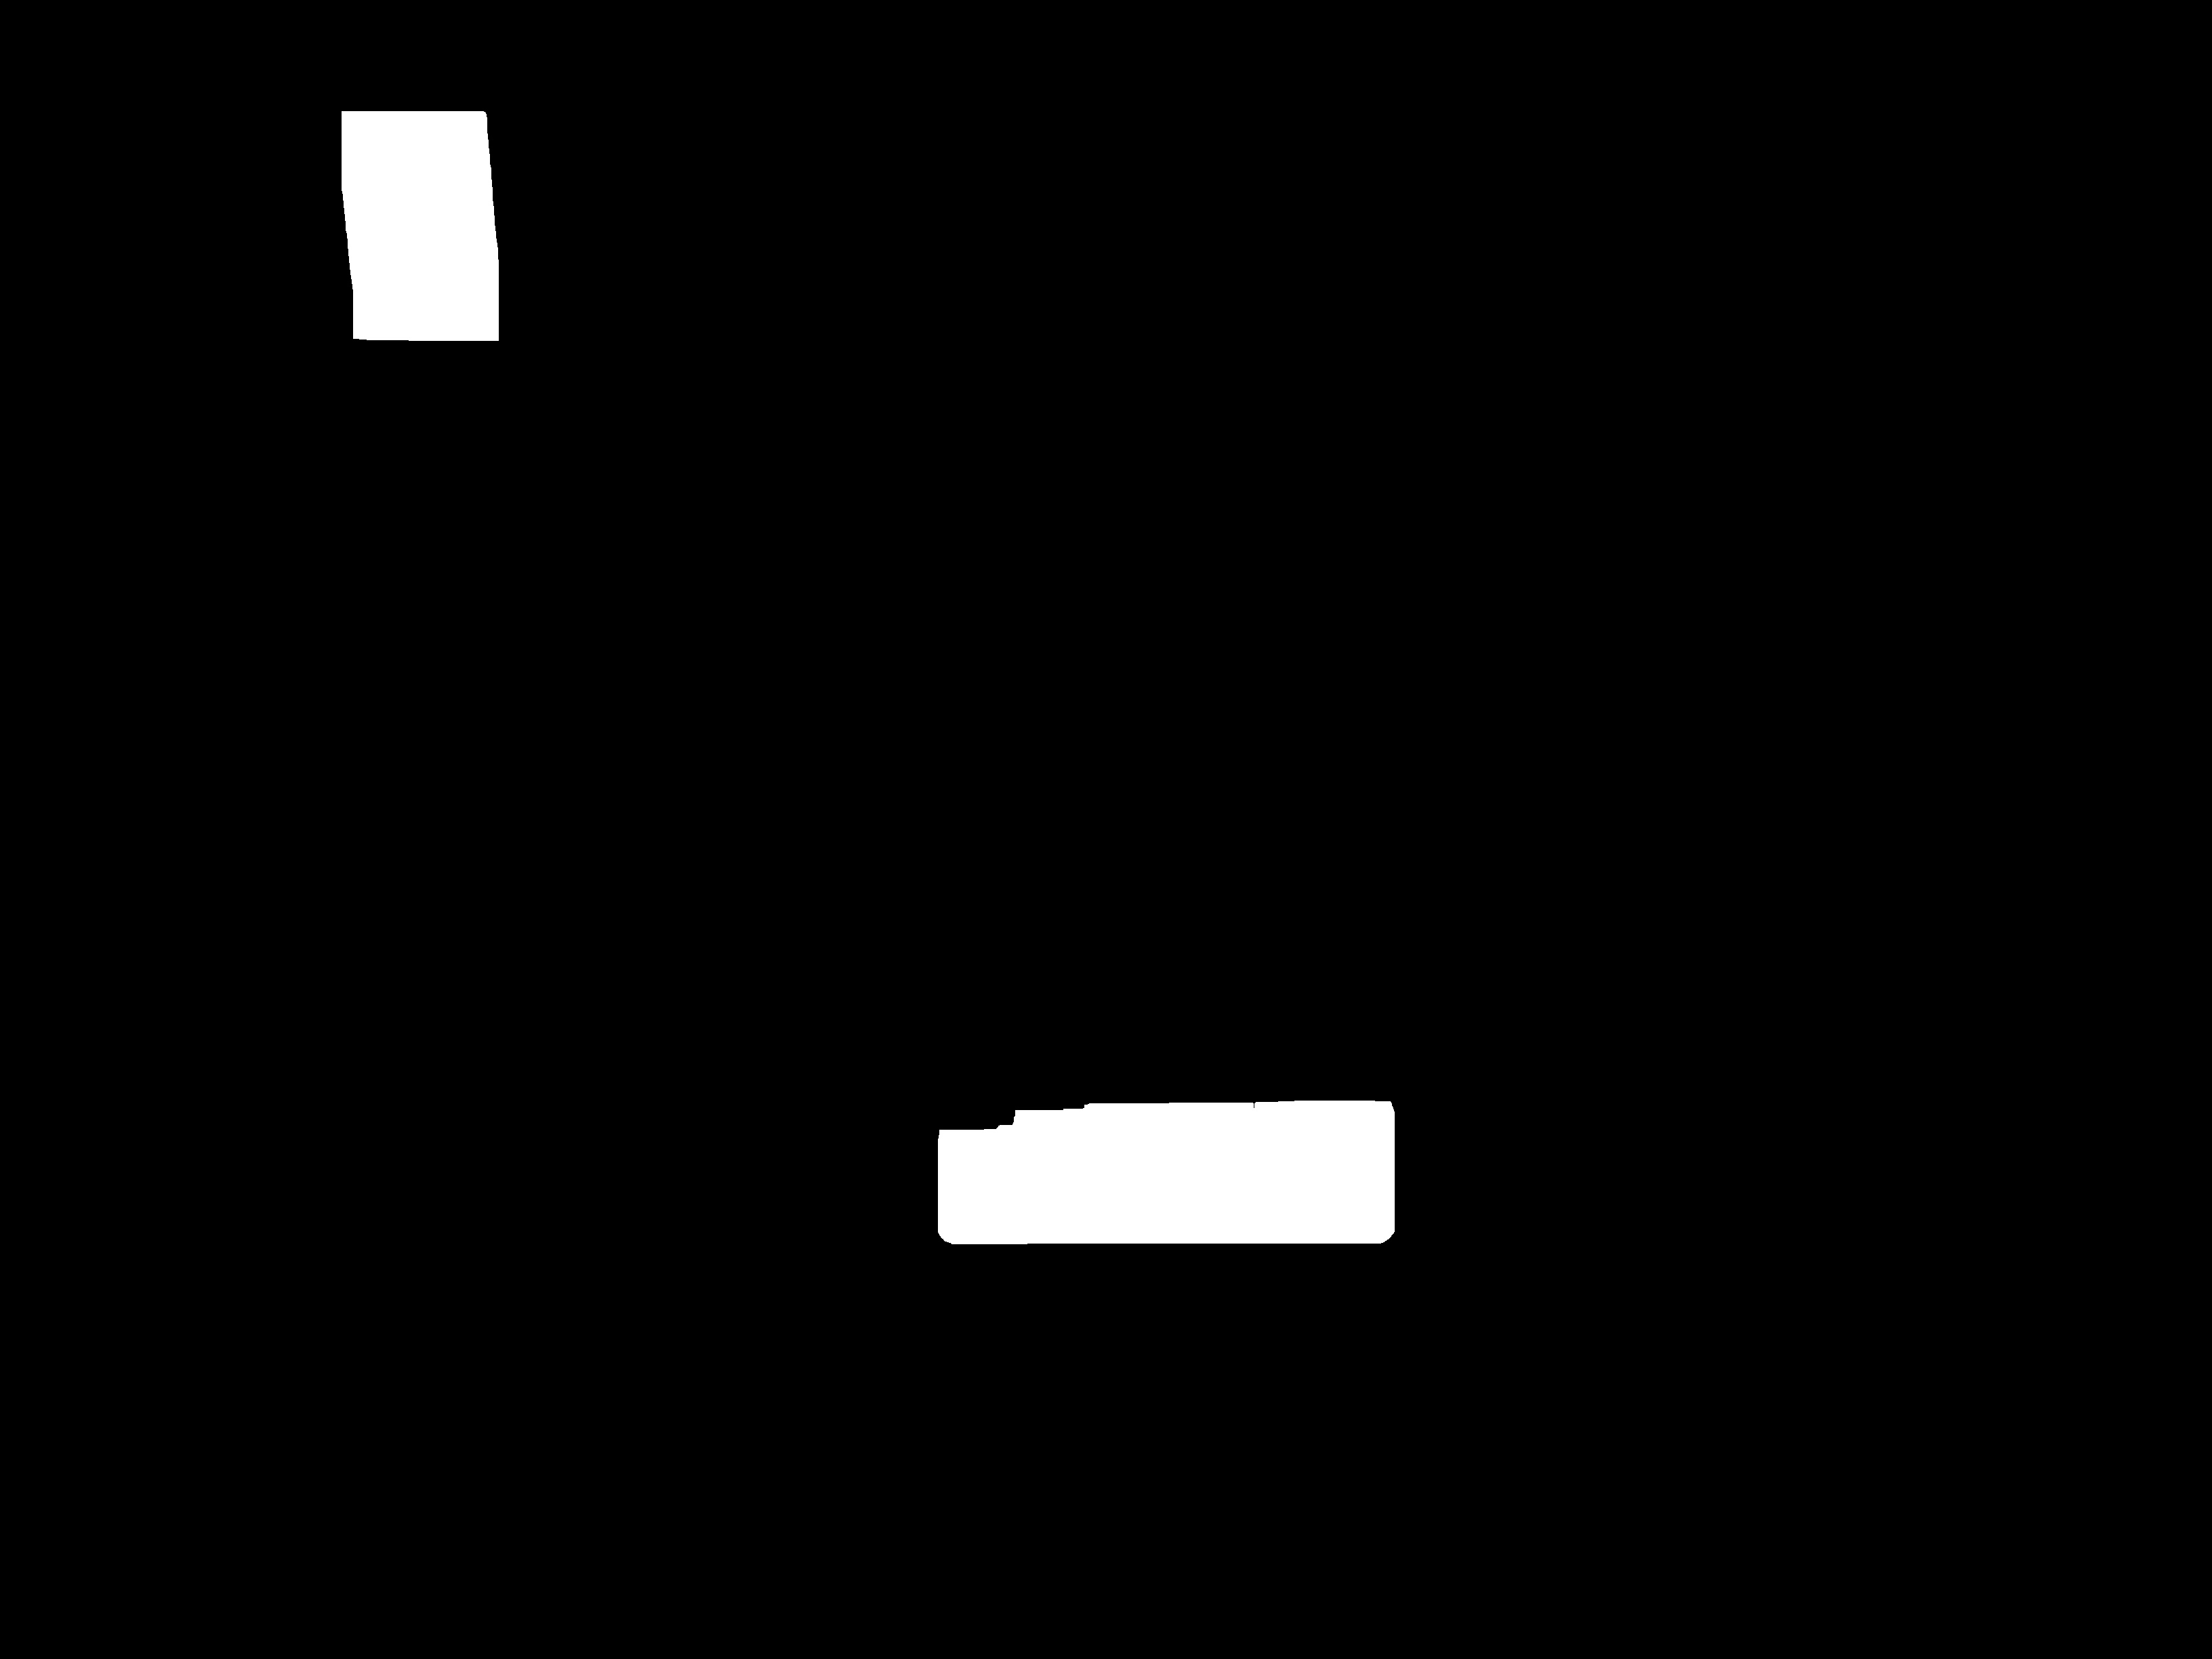
\includegraphics[width=88mm]{9fill_dilated.jpg}
	\caption{Detecção das áreas candidatas da placa}
	\label{fig:ext_plate_area_detection}
\end{figure}

\subsection{Extração da área da placa real}

Ao localizar as regiões candidatas, pode-se tanto encontrar uma placa, quanto regiões falsas, onde não existe placa. Para excluir estas regiões, Jia~\cite{jia2007region} sugere que características sejam extraídas para diferenciar corretamente as regiões de placa por outras. 

Diversas características podem ser utilizadas com este propósito. Elas incluem o tamanho da região, a altura e largura da região, a orientação dos caracteres posteriormente extraídos, a intensidade das bordas e a posição da região. 
 
Após a detecção da área da placa, essa área é extraída da imagem. Então os índices de linha e coluna da área da placa são encontrados por análise de componentes conectados. Na Figura~\ref{fig:ext_true_number_plate} podemos ver a imagem placa extraída da imagem original.

\begin{figure}[H]
	\centering
	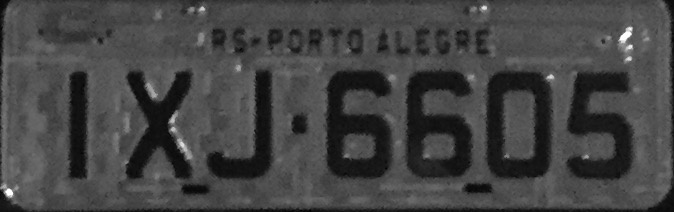
\includegraphics[width=88mm]{a01grayscale.jpg}
	\caption{Placa extraída}
	\label{fig:ext_true_number_plate}
\end{figure}

\subsection{Aprimoramento da região extraída}

A placa extraída deve ser convertida para um formato que seja processável pelo algoritmo. É aplicada sobre a imagem a conversão para tons de cinza seguida pela binarização. Apesar de a placa binarizada conter bastante ruído, não são feitas mais operações sobre a imagem da placa. O método seguinte, de segmentação de caracteres, Seção~\ref{sec:segmentacao}, vai lidar com os ruídos. O motivo da não utilização de algoritmos de remoção de ruído é para não deformar os caracteres a serem lidos pelo reconhecedor de caracteres na Seção~\ref{sec:reconhecimento}. A placa aprimorada e pronta para segmentação dos caracteres pode ser vista em~\ref{fig:ext_enhanced_number_plate}.

\begin{figure}[H]
	\centering
	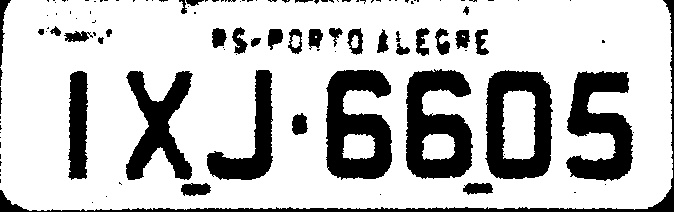
\includegraphics[width=88mm]{a02fill_binary.jpg}
	\caption{Placa aprimorada}
	\label{fig:ext_enhanced_number_plate}
\end{figure}

\section{Segmentação dos caracteres}
\label{sec:segmentacao}

O terceiro passo para o reconhecimento da placa é a segmentação dos caracteres, a qual consiste na extração dos caracteres utilizando
estratégias como projetar as suas informações de cores, rotulá-los ou comparar suas posições com modelos. A placa extraída no passo anterior pode conter
problemas de inclinação ou iluminação, mas o algoritmo de segmentação deve
superar todos esses problemas com pré-processamento~\cite{s2013automatic}.

Os principais algoritmos utilizados para a segmentação de caracteres são: segmentação utilizando conectividade de \emph{pixels}, segmentação utilizando perfis de projeção, segmentação utilizando conhecimento anterior dos caracteres, segmentação utilizando contorno dos caracteres e segmentação utilizando características combinadas~\cite{s2013automatic}.

O método une a segmentação utilizando a conectividade de \emph{pixels} com algum conhecimento anterior dos caracteres. É feita uma detecção de \emph{pixels} conectados para detectar quais elementos são possíveis caracteres e aplicando o conhecimento sobre a placa para descartar pontos muito pequenos ou muito próximos às bordas da placa.

O primeiro passo é o preenchimento dos espaços em branco da placa previamente tratada. Este passo existe para evitar que, ao detectar os contornos dos caracteres por meio da conexão dos \emph{pixels}, não aconteça uma dupla detecção em caracteres que contenham espaços internos abertos. Por exemplo o número 0, que possui um contorno interno e um contorno externo. Na Figura~\ref{fig:preenchimento} é possível ver a placa com os caracteres preenchidos por este passo.

\begin{figure}[H]
	\centering
	
\includegraphics[width=100mm]{b10filled_characters.png}
	\caption{Preenchimento dos caracteres}
	\label{fig:preenchimento}
\end{figure}

Neste ponto são detectados os contornos com base na conexão dos \emph{pixels}. Muitos \emph{pixels} conectados não fazem parte de nenhum caractere da placa. Para descartar os \emph{pixels} indesejados, é feito um filtro baseado no tamanho dos contornos e na sua posição. A altura dos contornos não pode ser menor do que metade da altura da imagem completa. Isso descarta os conjuntos pequenos de \emph{pixels} indesejados. Outro critério é que o contorno encontrado não pode estar encostado na borda da imagem. Em uma placa corretamente extraída os caracteres nunca vão estar encostando na borda. Este critério exclui sombras ou áreas que sobram na lateral da placa na extração, que poderiam ser erroneamente confundidas com caracteres.

\begin{figure}[H]
	\centering
	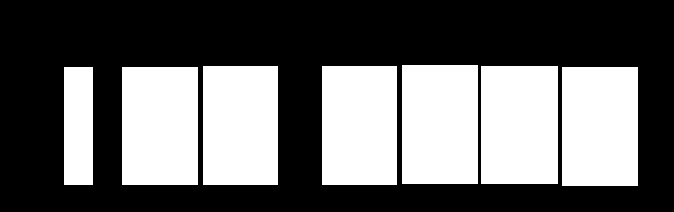
\includegraphics[width=100mm]{b20mask.png}
	\caption{Máscara gerada}
	\label{fig:mascara}
\end{figure}

Encontrados os contornos dos caracteres corretos, uma máscara, mostrada na Figura~\ref{fig:mascara}, é feita a partir deles. Essa máscara será aplicada sobre a imagem da placa extraída original, recortando os \emph{pixels} marcados por ela. Os caracteres recortados por essa operação serão extraídos, ordenados com base em sua posição x, e enviados para a etapa de reconhecimento de caracteres. A Figura~\ref{fig:caracteres_extraidos} mostra os caracteres a serem extraídos. 

\begin{figure}[H]
	\centering
	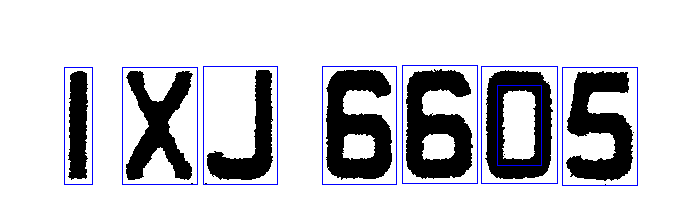
\includegraphics[width=100mm]{a08character_borders.png}
	\caption{Caracteres a serem extraídos}
	\label{fig:caracteres_extraidos}
\end{figure}

\section{Reconhecimento dos caracteres} \label{sec:reconhecimento}

O último passo para identificar a placa é o reconhecimento ótico dos
caracteres extraídos. Um dos maiores desafios da extração de caracteres é o fato de
os caracteres extraídos não terem o mesmo tamanho e espessura, devido ao
\emph{zoom} da câmera. Outro problema, ao criar um reconhecedor de propósito
geral, é a variedade nas fontes das placas ao redor do mundo~\cite{s2013automatic}. Este segundo problema não será um obstáculo para este trabalho pois só há interesse em reconhecer placas brasileiras. Outro desafio é o reconhecimento de caracteres semelhantes, como o D e o
0~\cite{ho2016intelligent}. Esse problema será mitigado com o conhecimento
prévio das placas brasileiras, uma vez que se sabe onde é possível haver letras e onde é possível haver números.

Tendo em mente os possíveis problemas, foi implementado um reconhecedor de caracteres especificamente para a solução deste problema. Foi utilizado o algoritmo \emph{K-Nearest Neighbors} para classificar os caracteres possíveis e utilizados os caracteres na fonte \emph{Mandatory} dispostos na Figura~\ref{fig:tipografia} como dados de treinamento. O \emph{feature space} consiste em um caractere apenas por classe, portanto é utilizado apenas um vizinho para classificar o novo dado.

Além de focar na fonte na qual as placas estão escritas, o reconhecedor é calibrado também para o padrão. Sabendo que a placa de trânsito tem três letras e quatro números, mantendo esta ordem, o reconhecedor nunca vai confundir uma letra com um número. Para conseguir este resultado são utilizados dois diferentes \emph{feature spaces}, um para os números e um para as letras. Assim, um caractere novo só pode ser classificado entre os possíveis candidatos.

Para que a classificação tenha sucesso, tanto as imagens de teste quanto as imagens a serem classificadas devem ter o mesmo tamanho. O \emph{feature space} deve ter \emph{N} dimensões não variáveis. Para isso as imagens são tratadas para que tenham todas o tamanho de 100x100 \emph{pixels}, preenchendo o espaço restante com \emph{pixels} brancos.

\begin{figure}[H]
	\centering
	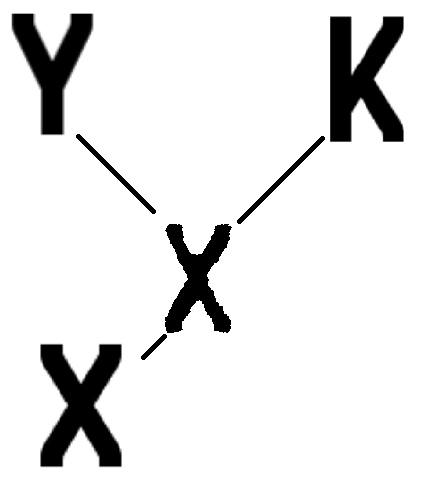
\includegraphics[width=50mm]{classificacao.png}
	\caption{Exemplo de classificação de caractere extraído}
	\label{fig:classificacao}
\end{figure}

Na Figura~\ref{fig:classificacao} são mostrados os três vizinhos mais próximos de um determinado caractere retirado do processamento de uma imagem. A sua projeção visual é hipotética e foi criada para representar de uma forma mais didática a seleção dos vizinhos. Pode-se reparar a semelhança entre os caracteres e entender porque eles foram selecionados pelo algoritmo ao visualizar a imagem.

\section{Otimização com Multiprocessamento em Pipeline} \label{sec:otimizacao}

Ao se processar imagens em um sistema embarcado, é preciso analisar e se adaptar às limitações do sistema. O computador \emph{Raspberry Pi} é bastante limitado, possuindo um processador \emph{Quad Core 1.2GHz Broadcom BCM2837 64bit CPU}. Por essa razão, para maximizar o ganho, foi nescessário utilizar técnicas de otimização. Dado o fato de ele possuir um \emph{Quad Core}, contendo quatro núcleos, é possível executar quatro processos em pararelo sem perder desempenho. 

A técnica utilizada na extração da placa e reconhecimento dos caracteres é uma técnica sequencial, que segue uma série de passos. Sabendo disso, é possível implementar um \emph{Pipeline} de execução. Um \emph{Pipeline} é um conjunto de elementos de processamento de dados conectados em série, onde a saída de um elemento é a entrada do próximo. \emph{Pipelines} podem ser executados em paralelo, pois o processamento de um não depende do outro.

As etapas de processamento de uma imagem foram divididas em quatro partes com tempo de processamento semelhante. Essas quatro etapas vão ser processadas cada uma em um núcleo diferente do processador do \emph{Raspberry Pi}, otimizando o seu tempo. O \emph{Pipeline} pode ser visto na maravilhosa tabela feita pelo matth abaixo:

Com a utilização do \emph{Pipeline}, o tempo de processamento da primeira imagem vai continuar o mesmo, mas para as próximas imagens, o tempo de processamento de cada uma será o tempo do etapa mais lenta entre as quatro, desconsiderando o tempo da comunicação entre os processos.

Os quatro processos foram divididos como se segue:

\begin{enumerate}
	\item O primeiro processo compreende desde a aquisição da imagem até a aplicação do filtro bilateral.
	\item O segundo processo compreende desde a equalização do histograma até o preenchimento dos espaços.
	\item O terceiro processo apenas executa a abertura morfológica.
	\item O quarto processo compreende desde o fechamento morfológico até o reconhecimento dos caracteres.
\end{enumerate}

Os procedimentos mais lentos são a aplicação do filtro bilateral e as operações de abertura e fechamento, por isso foram divididos em processos diferentes. Os demais procedimentos foram também divididos de forma que os processos tenham tempo de processamento semelhante.


















